\documentclass[12pt,a4paper]{article}
\usepackage{amstext}
\usepackage{fancyhdr}
\usepackage{amsfonts,graphicx,bezier, amssymb}
\usepackage{amsmath}
\usepackage{caption}
\usepackage{mathtools}
\usepackage{fancyhdr}
\usepackage{float}
\usepackage{authblk}
\usepackage[utf8]{inputenc}
\usepackage{pdflscape, lipsum, geometry}
\usepackage{pgfplots}
 \pgfplotsset{compat = newest}

%\usepackage[symbol]{footmisc}
%\renewcommand{\thefootnote}{\fnsymbol{footnote}}
\newcommand{\noi}{\noindent}
\newtheorem{thm}{Theorem}[section]
\newtheorem{defn}{Definition}[section]
\newtheorem{que}{Question}[section]
\newtheorem{rem}{Remark}[section]
\newtheorem{lm}{Lemma}[section]
\newtheorem{ex}{Example}[section]
\newtheorem{cor}{Corollary}[section]
\newtheorem{prop}{Proposition}[section]
\newenvironment{prf}{\noindent{\bf{Proof:}}~~}{\hfill\rule{1ex}{1ex}\vskip1.5ex}
\newcommand*\samethanks[1][\value{footnote}]{\footnotemark[#1]}
\newenvironment{Rem}{\noindent{\bf{Remark:}}~~}{\hfill\rule{1ex}{1ex}\vskip1.5ex}
\usepackage{tikz}
\usepackage{color}
\usetikzlibrary{matrix}
\newcommand*\circled[1]{\tikz[baseline=(char.base)]{
		\node[shape=circle,draw,inner sep=1pt] (char) {#1};}}

%\usepackage[colorlinks]{hyperref}
\begin{document}
	\tikzset{ 
		table/.style={
			matrix of nodes,
			row sep=-\pgflinewidth,
			column sep=-\pgflinewidth,
			nodes={
				rectangle,
				draw=black,
				align=center
			},
			minimum height=0.5em,
			text depth=4.0ex,
			text height=2ex,
			nodes in empty cells,
			
			every even row/.style={
				nodes={fill=gray!20}
			},
			column 1/.style={
				nodes={text width=1em,font=\bfseries}
			},
			row 1/.style={
				nodes={
					fill=white,
					text=black,
					font=\bfseries
				}
			}
		}
	}
	
	
	
	
	%\begin{figure}[!h]
	% 		\begin{tikzpicture}[scale=1]
		
		\begin{center}\Large{\bf{Reduced submodules of finite dimensional polynomial modules}}
			
		\end{center}
		\vspace*{0.3cm}
		\begin{center}
			
			
			
			
			Tilahun Abebaw \footnote{Department of Mathematics, Addis Ababa University, P. O. BOX 1176, Addis Ababa, Ethiopia, teklemichael.worku@aau.edu.et, tilahun.abebaw@aau.edu.et}, Nega Arega\footnote {Department of Mathematics and Statistics, The Namibia University of Science and Technology, Namibia,  nechere@nust.na},
			Teklemichael Worku Bihonegn\footnotemark[1] \footnote{This work forms part of the third author's PhD thesis}, Dominic Bunnett\footnote{Institute for Mathematics, Berlin, Germany, dominic.bunnett@googlemail.com},
			David Ssevviiri\footnote[5]{Department of Mathematics, Makerere University, P. O. BOX 7062, Kampala, Uganda, david.ssevviiri@mak.ac.ug} \footnote[6] {Corresponding author.}
		\end{center}
		
		\begin{abstract}
			Let $k$ be a field, $R$ be the ring $k[x, y]$ and $I$ be a monomial ideal of $R$. Using combinatorics (in particular Young diagrams), we characterize, classify and give a geometric interpretation of the largest reduced submodules, $\mathfrak{R}(M)$ of the $R$-modules, $M:=R/I$ which when considered as $k$-modules are finite dimensional.
			
		\end{abstract}
		
		{\bf Keywords}: Reduced modules, Young diagrams, finite dimensional modules.   
		
		\vspace*{0.4cm}
		
		{\bf MSC 2010}  : 16D70, 16D80, 05E40, 16D60, 13C60
		\section{Introduction}
		\begin{paragraph}\noi
			Reduced rings play an important role in algebra. A module analogue of reduced rings was first defined by Lee and Zhou in \cite{lee2004reduced}. Reduced modules have since been studied by \cite{agayev2009reduced, kyomuhangi2020locally, rege2008reduced, ssevviiri2022applications} among others.
			Let $R$ be a commutative unital ring. Let $I$ be an ideal of $R$. Among other applications, reduced modules form a full subcategory of $R$-Mod on which the $I$-torsion functor $\Gamma_I$ is representable, i.e., if $M$ is an $I$-reduced $R$-module, then $\Gamma_I(M)\cong \text{Hom}(R/I, M)$, see \cite{ssevviiri2022applications}. It was shown in \cite{ssevviiri2022applications} that reduced modules and their dual, coreduced modules provide a setting in which both the MGM equivalence and Greenless-May duality hold. A more general version of reduced modules was studied recently in \cite{kyomuhangi2021generalised}. We note that this is what Rohrer and Yekutieli studied in \cite{rohrer2019torsion} and \cite{yekutieli2021weak} respectively, although instead called them modules with bounded torsion. The same modules are called modules whose submodules $(0:_M a^t)$ with $a \in R$ and $t\in \mathbb{Z}^+$ are stationary, by Schenzel and Simon in \cite[Proposition $3.1.10$]{schenzel2018completion}. This general version of reduced modules relates to prisms which belong to the groundbreaking theory of perfectoid rings, \cite{bhatt2019prisms, yekutieli2021weak}.
		\end{paragraph}
		\begin{defn}
			An $R$-module $M$ is {\it reduced} if for all $a\in R$ and $m\in M,~ a^2m=0$ implies that $am=0$.
		\end{defn}
		\begin{paragraph}\noi
			We wish to study for an arbitrary $R$-module $M$ in a suitable full  subcategory of $R$-Mod, the category of $R$-modules, the set
			\begin{equation}
				\mathfrak{R}(M):=\{m\in M: a^2m=0 \Rightarrow am=0 ~\text{for~~all}~ a\in R\}.
			\end{equation} By definition, $M$ is a reduced $R$-module if and only if $\mathfrak{R}(M)=M$. It is easy to see that in general $\mathfrak{R}(M)$ is not a submodule of $M$. However, it is a submodule under special cases. For example see \cite[Theorem 2.1]{ssevviiri2012structure}. 
		\end{paragraph}
		%	where $R:=\mathbb{Z}$, the ring of integers and $M:=\mathbb{Z}/p^{k_1}_1\mathbb{Z} \times \cdots \times \mathbb{Z}/p^{k_n}_n\mathbb{Z}$, where $p_i$ are prime numbers and $k_i \in \mathbb{Z}^+$; $\mathfrak{R}(M)$ is a submodule of $M$ given by $\{0\} \cup \{m p_1^{k_1-1} \times \cdots \times p_n^{k_n-1}\}_{m=1}^{p_1 p_2 \cdots p_n-1}$.
		\begin{paragraph}\noi
			Let $k$ be a field and $R:=k[x, y]$. In this paper, we characterize, classify and give a geometric interpretation of reduced submodules, $\mathfrak{R}(M)$ of $R$-modules $M$ in the full subcategory $\mathfrak{C}$ of $R$-Mod given by $$\text{\Large $\mathfrak{C}$}:=\bigg\{ M \in R\text{-Mod} ~|~ M=R/I,~ I~\text{is a monomial ideal of $R$ and} ~\text{dim}_k  (R/I)  < \infty\bigg\}.$$
			The methods employed are combinatorial. In particular, we use Young diagrams. A Young diagram is defined as a collection of boxes or cells arranged in left-justified rows, with a (weakly) decreasing number of boxes in each row. 
		\end{paragraph}
		\begin{paragraph}\noi
			Let $n\in \mathbb{Z}^+$. A {\it partition} of $n$ written as $(\lambda_1, \lambda_2, \cdots, \lambda_k)$ is a sequence of nonnegative integers $\lambda_1, \lambda_2,\cdots,\lambda_k$ such that $\lambda_1+ \lambda_2+\cdots+\lambda_k=n$. To a partition $\lambda=(\lambda_1, \lambda_2, \cdots, \lambda_k)$ of $n$ is associated a Young diagram
			
			$$	\begin{tikzpicture}[scale=0.5]
				\draw [-] (0, 0) -- (1, 0);
				\draw [-] (0, 0) -- (0, 4);
				\draw [-] (1, 0) -- (1, 4);
				\draw [-] (2, 1) -- (2, 4);
				\draw [-] (3, 2) -- (3, 4);
				\draw [-] (4, 3) -- (4, 4);
				\draw [-] (0, 1) -- (2, 1);
				\draw [-] (0, 2) -- (3, 2);
				\draw [-] (0, 3) -- (4, 3);
				\draw [-] (0, 4) -- (4, 4);
				
				\node (p) at (-0.5, 3.5) {$\lambda_1$};
				\node (p) at (-0.5, 2.5) {$\lambda_2$};
				\node (p) at (-0.5, 1.5) {$\vdots$};
				\node (p) at (-0.5, 0.5) {$\lambda_k$};
			\end{tikzpicture}$$
			
			with $\lambda_i$ boxes in the $i^{th}$ row of boxes lined up on the left. Partitions and their corresponding Young diagrams encode information about many phenomena in Mathematics. For instance; they are in a one-to-one correspondence with conjugacy classes of the symmetric groups $S_n$ and with their corresponding irreducible representations   \cite{fulton1997young, fulton1991}. They also encode information about ideals in the Hilbert schemes of points on a surface \cite{nakajima1999lectures}.
		\end{paragraph}
		\newpage
		\begin{paragraph}\noi
			In Section $2$, we show that 
			for any $M\in \mathfrak{C}$, the set $\mathfrak{R}(M)$ defined in Equation $(1)$:
			\begin{itemize}
				\item  is a submodule of $M$,
				\item  is the largest reduced submodule of $M$,
				\item  is generated by all elements at the sharp points of the Young diagram associated to $M$,
				\item  coincides with both $\text{Soc}(M)$, the socle of $M$ and the submodule $(0 :_M \{x, y\})$, the collection of all elements of $M$ annihilated by the ring elements $\{x, y\}$. 
			\end{itemize}
			It is also shown that if $M\in \mathfrak{C}$ and ${\bf x}=x, y$ is a sequence of elements of the ring $R:=k[x, y]$, then the Koszul cohomologies $H^i(x, y;M)$ are all reduced $R$-modules.
		\end{paragraph}
		\begin{paragraph}\noi
			In Section $3$, we classify the submodules $\mathfrak{R}(M)$ of modules $M$, for which $\text{dim}_kM=n<\infty$ into four. The classification is based on the structure of the submodule $\mathfrak{R}(M)$.
			In the last section of the paper, Section $4$, we give a geometric interpretation of $\mathfrak{R}(M)$ for any $M \in \mathfrak{C}$ in terms of  the Hilbert scheme of points on a surface.
		\end{paragraph}
		
		
		
		
		\section{Characterization}
		\begin{paragraph}\noi
			The $k$-algebra $R:=k[x, y]$ takes the form of Figure $1$ when represented on the grid. If the monomial ideal $I$ of $k[x, y]$ is given by, $I:=\langle x^5, x^4y, x^3y^2, x^2y^3, xy^5, y^7 \rangle$, then this ideal is represented by the unshaded region in Figure $1$. It follows that the quotient $k$-module $M=\frac{k[x, y]}{I}$ is finite dimensional with dimension  $18$ and is generated by elements in the shaded region. All modules $M\in \mathfrak{C}$ can be represented on a Young diagram. For $M$ in Figure $1$, $\mathfrak{R}(M)=\frac{J}{I}$, where $J=\langle x^4, x^3y, x^2y^2, xy^4, y^6 \rangle$. Note that $\text{dim}_kM=1$ if and only if $M\cong k$ in which case  $\mathfrak{R}(M)=M$. $\text{dim}_kM=2$ if and only if $M=k[x]/\langle x^2 \rangle$ or $M=k[y]/\langle y^2 \rangle$, so that $\mathfrak{R}(M)=\langle x \rangle/\langle x^2\rangle$ or $\langle y \rangle/\langle y^2\rangle$ respectively. For more examples of $\mathfrak{R}(M)$, for $M$ with $k\text{-dim}, 3, 4, 5, 6$ and $7$ see Figures $2, 3, 4, 5$ and $6$ respectively.
		\end{paragraph}
		\begin{lm}
			Let $M\in \mathfrak{C}$. For any $m$ in the generating set of $M$ and $a\in \langle x, y\rangle$, there exists $t\in \mathbb{Z}^+$  such that $a^tm=0$.
		\end{lm}
		\begin{prf}
			If $am=0$, we are done. Suppose that $am \neq 0$. We get $4$ cases. The first $3$ cases include: $a$ is a scalar multiple of $x, a$ is a scalar multiple of $y$ and $a$ is a scalar multiple of $xy$. Raising $a$ to a positive integer $t$, moves $m$ to $a^tm$ along a row, along a column and diagonally respectively, in the Young diagram associated to $M$. If $t$ is sufficiently large, then $a^tm=0$. The fourth case is when $a$ is a linear combination of any of the $3$ cases mentioned above. Still when it is raised to $a$ sufficiently large $t$, it is easy to see that even in this case $a^tm=0$.
		\end{prf}
		\begin{figure}[H]
			
			$$	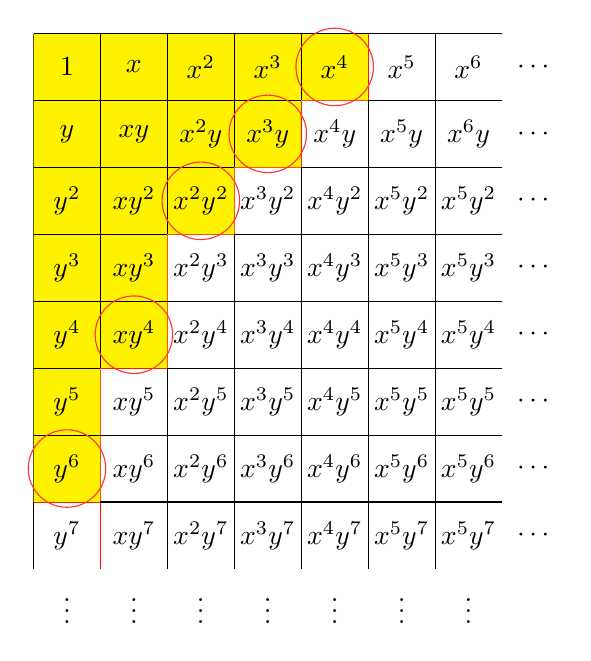
\begin{tikzpicture}[scale=0.85][thick]
				%\draw [-] (0, 0) -- (7, 0);
				\draw [-] (0, 0) -- (0, 8);
				\draw [red] (0, 1) -- (1, 1);\draw [red] (1, 1) -- (1, 3);\draw [red] (1, 3) -- (2, 3);\draw [red] (2, 3) -- (2, 5);\draw [red] (2, 5) -- (3, 5);\draw [red] (3, 5) -- (3, 6);\draw [red] (3, 6) -- (4, 6);
				\draw [red] (4, 6) -- (4, 7);
				\draw [red] (5, 7) -- (5, 8);
				\draw [red] (4, 7) -- (5, 7);
				\draw [red] (1, 0) -- (1, 1);
				\fill [yellow ]  (0, 1) --  (0, 8) rectangle (1, 1) -- (1, 8);
				\fill [yellow ] (2, 5) --  (2, 8) rectangle (3, 5) -- (3, 8);
				\fill [yellow  ] (1, 3) --  (1, 8) rectangle (2, 3) -- (2, 8);
				\fill [yellow ] (3, 6) --  (3, 8) rectangle (4, 6) -- (4, 8);
				\fill [yellow ] (4, 7) --  (5, 7) rectangle (4, 8) -- (5, 8);
				\draw [-] (1, 3) -- (1, 8);
				\draw [-] (2, 0) -- (2, 3);
				\draw [-] (2, 5) -- (2, 8);
				\draw [-] (3, 0) -- (3, 5);
				\draw [-] (3, 6) -- (3, 8);
				\draw [-] (4, 0) -- (4, 6);
				\draw [-] (4, 7) -- (4, 8);
				\draw [-] (5, 0) -- (5, 7);
				\draw [-] (6, 0) -- (6, 8);
				%\draw [-] (7, 0) -- (7, 8);
				\draw [-] (1, 1) -- (7, 1);
				\draw [-] (0, 2) -- (7, 2);
				\draw [-] (0, 3) -- (1, 3);\draw [-] (2, 3) -- (7, 3);
				\draw [-] (0, 4) -- (2, 4);\draw [-] (2, 4) -- (7, 4);
				\draw [-] (0, 5) -- (2, 5);\draw [-] (3, 5) -- (7, 5);
				\draw [-] (0, 6) -- (3, 6);\draw [-] (4, 6) -- (7, 6);
				\draw [-] (0, 7) -- (4, 7);\draw [-] (5, 7) -- (7, 7);
				\draw [-] (0, 8) -- (7, 8);
				
				\node (p) at (0.5, 7.5) {1};
				\node (p) at (1.5, 7.5) {$x$};
				\node (p) at (2.5, 7.5) {$x^2$};
				\node (p) at (3.5, 7.5) {$x^3$};
				\node[circle, draw=red!80, inner sep=0pt, minimum size=28pt] ($x^4$) at (4.5, 7.5) {$x^4$};
				\node (p) at (5.5, 7.5) {$x^5$};
				\node (p) at (6.5, 7.5) {$x^6$};
				\node (p) at (7.5, 7.5) {$\cdots$};
				
				\node (p) at (0.5, 6.5) {$y$};
				\node (p) at (1.5, 6.5) {$xy$};
				\node (p) at (2.5, 6.5) {$x^2y$};
				\node[circle, draw=red!80, inner sep=0pt, minimum size=28pt] ($x^3y$) at (3.5, 6.5) {$x^3y$};
				\node (p) at (4.5, 6.5) {$x^4y$};
				\node (p) at (5.5, 6.5) {$x^5y$};
				\node (p) at (6.5, 6.5) {$x^6y$};
				\node (p) at (7.5, 6.5) {$\cdots$};
				
				\node (p) at (0.5, 5.5) {$y^2$};
				\node (p) at (1.5, 5.5) {$xy^2$};
				\node[circle, draw=red!80, inner sep=0pt, minimum size=28pt] ($x^2y^2$) at (2.5, 5.5) {$x^2y^2$};
				\node (p) at (3.5, 5.5) {$x^3y^2$};
				\node (p) at (4.5, 5.5) {$x^4y^2$};
				\node (p) at (5.5, 5.5) {$x^5y^2$};
				\node (p) at (6.5, 5.5) {$x^5y^2$};
				\node (p) at (7.5, 5.5) {$\cdots$};
				
				\node (p) at (0.5, 4.5) {$y^3$};
				\node (p) at (1.5, 4.5) {$xy^3$};
				\node (p) at (2.5, 4.5) {$x^2y^3$};
				\node (p) at (3.5, 4.5) {$x^3y^3$};
				\node (p) at (4.5, 4.5) {$x^4y^3$};
				\node (p) at (5.5, 4.5) {$x^5y^3$};
				\node (p) at (6.5, 4.5) {$x^5y^3$};
				\node (p) at (7.5, 4.5) {$\cdots$};
				
				\node (p) at (0.5, 3.5) {$y^4$};
				\node[circle, draw=red!80, inner sep=0pt, minimum size=28pt] ($xy^4$) at (1.5, 3.5) {$xy^4$};
				\node (p) at (2.5, 3.5) {$x^2y^4$};
				\node (p) at (3.5, 3.5) {$x^3y^4$};
				\node (p) at (4.5, 3.5) {$x^4y^4$};
				\node (p) at (5.5, 3.5) {$x^5y^4$};
				\node (p) at (6.5, 3.5) {$x^5y^4$};
				\node (p) at (7.5, 3.5) {$\cdots$};
				
				\node (p) at (0.5, 2.5) {$y^5$};
				\node (p) at (1.5, 2.5) {$xy^5$};
				\node (p) at (2.5, 2.5) {$x^2y^5$};
				\node (p) at (3.5, 2.5) {$x^3y^5$};
				\node (p) at (4.5, 2.5) {$x^4y^5$};
				\node (p) at (5.5, 2.5) {$x^5y^5$};
				\node (p) at (6.5, 2.5) {$x^5y^5$};
				\node (p) at (7.5, 2.5) {$\cdots$};
				\node[circle, draw=red!80, inner sep=0pt, minimum size=28pt] ($y^6$) at (0.5, 1.5) {$y^6$};
				\node (p) at (1.5, 1.5) {$xy^6$};
				\node (p) at (2.5, 1.5) {$x^2y^6$};
				\node (p) at (3.5, 1.5) {$x^3y^6$};
				\node (p) at (4.5, 1.5) {$x^4y^6$};
				\node (p) at (5.5, 1.5) {$x^5y^6$};
				\node (p) at (6.5, 1.5) {$x^5y^6$};
				\node (p) at (7.5, 1.5) {$\cdots$};
				
				\node (p) at (0.5, 0.5) {$y^7$};
				\node (p) at (1.5, 0.5) {$xy^7$};
				\node (p) at (2.5, 0.5) {$x^2y^7$};
				\node (p) at (3.5, 0.5) {$x^3y^7$};
				\node (p) at (4.5, 0.5) {$x^4y^7$};
				\node (p) at (5.5, 0.5) {$x^5y^7$};
				\node (p) at (6.5, 0.5) {$x^5y^7$};
				\node (p) at (7.5, 0.5) {$\cdots$};
				
				\node (p) at (0.5, -0.5) {$\vdots$};
				\node (p) at (1.5, -0.5) {$\vdots$};
				\node (p) at (2.5, -0.5) {$\vdots$};
				\node (p) at (3.5, -0.5) {$\vdots$};
				\node (p) at (4.5, -0.5) {$\vdots$};
				\node (p) at (5.5, -0.5) {$\vdots$};
				\node (p) at (6.5, -0.5) {$\vdots$};
			\end{tikzpicture}$$
			\caption{Generators for $\mathfrak{R}(M)$ and $M$ on a Young diagram.}
		\end{figure}
		
		
		\begin{paragraph}\noi
			For any ideal $I\subseteq k[x, y]$ and a $k[x, y]$-module $M, ~\Gamma_I(M)$ is the submodule of $M$ given by $\Gamma_I(M):=\big\{m\in M ~|~I^tm=0, ~\text{for~some}~t \in \mathbb{Z}^+ \big\}$.
		\end{paragraph}
		\begin{prop}
			\normalfont
			Let $M \in \mathfrak{C}$. For any monomial ideal $I$ of $k[x, y]$, $\Gamma_I(M)=M$. 
		\end{prop}
		\begin{prf}
			Any monomial ideal $I$ of $k[x, y]$ is contained in the maximal ideal $\langle x, y\rangle$ of $k[x, y]$. By Lemma $2.1$, there exists $k\in \mathbb{Z}^+$ such that $I^km_i=0$ for each generators $m_i$ of $M \in \mathfrak{C}$, then for any $m\in M$, $I^km=I^k\sum_{i}f_im_i=\sum_{i}f_iI^km_i=0$, where $f_i \in k[x, y]$, so $\Gamma_I(M)=M$.
		\end{prf}
		
		
		\begin{lm}
			\normalfont
			Let $M \in \mathfrak{C}$. If an element $m$ in the generating set of $M$ as a $k$-module is not at the sharp point of the Young diagram corresponding to $M$, then there exists $a \in \langle x, y\rangle$ such that $am \neq 0$.
		\end{lm}
		\begin{prf}
			If $m$ is in the $n^{th}$ column of the Young diagram associated to $M$ and the $n^{th}$ column is not the last column consisting of nonzero elements of $M$, then $xm\neq 0$. Since it will be in the $(n+1)^{th}$ column which must also contain nonzero element(s) of $M$ in the same row as that of $m$. A similar argument shows that $ym\neq 0$ when roles of a column are swapped with those of a row.
		\end{prf}
		\begin{lm}
			\normalfont
			Let $a\in k$ and $n\in M$, $n=am$, where $m$ is a nonzero element at the sharp point of a Young diagram corresponding to $M$ if and only if $xn=yn=0$.
		\end{lm}
		\begin{prf}
			If $m$ is at the sharp point of the Young diagram corresponding to $M$, then $m$ appears in the last row and last column for which elemnts of $M$ are nonzero. So, $xm$ and $ym$ is a shift through one step horizontally and one step vertically respectively which leads  into the zero of $M$. So, $xm=ym=0$ and therefore $xn=0=yn$. Conversely, suppose that $0\neq m\in M$ and $xam=0=yam$, since $a\in k$ and $R$ is commutative we have $xm=0=ym$. Since $m\neq 0$, $xm=0$ (resp. $ym=0$) implies that $m$ is in the last column (resp. row) of the Young diagram associated to $M$. So, $xn=yn=0$ implies that $m$ appears at the sharp point of the Young diagram.
		\end{prf}
		\begin{prop}
			\normalfont
			Let $M\in \mathfrak{C}$, $S:=\{m_1, m_2,\cdots, m_n\}$ be the collection of all elements in the generating set of $M$ that appear at the sharp points of the Young diagram corresponding to $M$ and $T$ the generating set of $M$. Then $$S=\mathfrak{R}(M) \cap T.$$
		\end{prop}
		\begin{prf}
			If $m\notin S$ and $m$ is in the generating set of $M$, then by Lemma $2.2$, there exists $a\in \langle x, y \rangle \subseteq k[x, y]$ such that $am \neq 0$. By Lemma $2.1$ there exists a positive integer $t$ such that $a^tm=0$. Thus, $m\notin \mathfrak{R}(M)$. So, if $T$ is the generating set of $M$, then $\mathfrak{R}(M) \cap T \subseteq S\cap T=S$. Now let $m\in S, a\in \langle x, y \rangle$ and $t\in \mathbb{Z}^+$ such that $a^tm=0$. By Lemma $2.3$ $am=0$, since $a$ is a linear combination of $x$ and $y$. If $a\in R\setminus \langle x, y \rangle$, then for any $0\neq m\in S$, $am\neq 0$ and $a^km \neq 0$ for all $k\in \mathbb{Z}^+$. This shows that $S\subseteq \mathfrak{R}(M) $. Since $S\subseteq T$, we have $S\subseteq \mathfrak{R}(M) \cap T$.
		\end{prf}
	\begin{lm}
		\normalfont
		Let $S$ be as defined in Proposition $2.2$ and $\langle S \rangle_k$, the $k$-submodule of $M$ generated by $S$, then $$\langle S \rangle_k \subseteq \mathfrak{R}(M).$$
	\end{lm}
	\begin{prf}
		Let $m\in \langle S \rangle_k$, i.e, $m=\sum_{i=1}^{n}r_im_i$ where $r_i \in k$ and $m_i \in S$. Suppose that $a^2m=0$ for some $a\in R$. If $a\in \langle x, y \rangle$, then $a$ is a linear combination of $x$ and $y$ and by Lemma $2.3~ar_im_i=0$ for all $i\in \{1, \cdots, n\}$. It follows that $am=\sum_{i=1}^{n}ar_im_i=0$. Now suppose that $a\in R\setminus \langle x, y \rangle$, $a=a_0+a_1x+a_2y+\cdots$. So, by Lemma $2.3$ $am=a_0r_im_i$ for all $i\in \{1, \cdots, n\}$, since $xm_i=0=ym_i$, for all $m_i\in S$. It follows that $a^2m=0$ implies that $a^2_0r_im_i=0$ for all $i\in \{1, \cdots, n\}$. Since $a_0, a^2 \in k$, multiplying $a_0$ or $a^2$ with each $r_im_i, r_im_i$ doesn't shift the cell. So, $a_0^2r_im_i=0$ if and only if $r_im_i=0$ if and only if $a_0r_im_i=0$ for all $i\in\{1, \cdots, n\}$. Thus, $a_0r_im_i=0$ implies that $am=0$. So, any $m\in \langle S \rangle_k$ also belongs to $\mathfrak{R}(M)$.
	\end{prf}
	\begin{thm}
		\normalfont
		Let $S$ and $T$ be as in Proposition $2.2$. For any $M\in \mathfrak{C}$, $$\langle S\rangle_k=\mathfrak{R}(M).$$
	\end{thm}
	\begin{prf}
		By Lemma $2.4 ~\langle S \rangle_k \subseteq \mathfrak{R}(M)$. Let $m\in \mathfrak{R}(M)\subseteq M$. Since $M$ is finitely generated, $m=\sum_{j=1}^{t}r_jm_j$ with each $m_j\in T$, $r_j\in k$ and $\langle T \rangle_k= M$. Without loss of generality, assume there exists $i\in \{1, \cdots, t\}$ such that $m_i\notin S$ but $m_j\in S$, for all $j\neq i$. Then $xm_i\neq 0$ and $ym_i\neq 0$, but $xm_j=0=ym_j=0$ for all $j\in \{1, \cdots, n\}\setminus \{i\}$. So, $xm=xr_1m_1+xr_2m_2+\cdots +xr_im_i+ \cdots +xr_km_k=xr_im_i \neq 0$. However, by Lemma $2.1$ there exists $l \in \mathbb{Z}^+$ such that $x^lm=x^lr_im_i=0$. This shows that $m\notin \mathfrak{R}(M)$ which is a contradiction. So, if $m\in \mathfrak{R}(M)$ and $m=\sum_{j=1}^{t}r_jm_j$, then each $m_j\in S$ and therefore
		$m\in \langle S \rangle_k$ and $\mathfrak{R}(M)\subseteq \langle S \rangle_k$. 
	\end{prf}
		\begin{cor}
			\normalfont
			Let $S$ be as in Proposition $2.2$. For any $M \in \mathfrak{C},~ \langle x,y \rangle \mathfrak{R}(M)=0$.
		\end{cor}
		\begin{prf}
			Let $m\in \mathfrak{R}(M)$. By Theorem $2.1$, $m=\sum_{i}a_im_i$, where $a_i\in k[x, y]$ and $m_i \in S$. However, from Lemma $2.3,~xm_i=ym_i=0$ for all $i$. It follows that $\langle x, y \rangle m=0$, for all $m\in \mathfrak{R}(M)$. So $\langle x,y \rangle \mathfrak{R}(M)=0$. 
		\end{prf}
		By $N\leq M$ we mean $N$ is a submodule of $M$.
		Define, 
		$$\text{\Large $\mathfrak{C}$}_\text{red}:=\bigg \{ N \leq M~ |~ M \in \mathfrak{C}~\text{and}~ N~ \text{is a reduced} ~R \text{-module} \bigg \}. $$
		$$\text{\Large $\mathfrak{C}$}_\text{semi}:=\bigg \{N \leq M~ |~ M \in \mathfrak{C}~\text{and}~ N~ \text{is  a semisimple } R\text{-module} \bigg \}.$$
		
		\begin{paragraph}\noi
			An $R$-module $M$ is said to be {\it $I$-torsion} (resp. {\it $I$-complete}, and {\it $I$-coreduced}) if $\Gamma_I(M)\cong M$ (resp. $\Lambda_I(M)\cong M$ and $\Lambda_I(M)\cong \frac{M}{IM}$). $I$-complete modules are a very old notion. $I$-coreduced is relatively new, see \cite{ssevviiri2022applications}. Equivalently, $M$ is $I$-coreduced if for every $a\in I$ and $m\in M$, there exists $n\in M$ such that $am=a^2n$.
		\end{paragraph}
		\begin{prop}
			\normalfont
			For any monomial ideal $I$ of $R:=k[x, y]$ and any $N\in \mathfrak{C}_\text{red}$, $N$ is:
			\begin{itemize}
				\item [1.]  $I$-torsion,
				\item [2.]  $I$-complete, and
				\item [3.] $I$-coreduced.
			\end{itemize}
		\end{prop}
		\begin{prf}
			Let $N\in \mathfrak{C}_\text{red}$. For any monomial ideal $I$ of $k[x, y]$ and $k\in \mathbb{Z}^+$,
			\begin{itemize}
				\item [1.] $I^k \subseteq \langle x, y \rangle$. By Corollary $2.1$, $I^kN \subseteq \langle x, y \rangle N=\langle x, y \rangle \mathfrak{R}(M)=0$,  thus $N \subseteq \Gamma_I(N)$.
				\item [2.] By \cite[Corollary $3.2$]{ssevviiri2022applications}, for $N \in \mathfrak{C}_\text{red},~ \Lambda_I(\Gamma_I(N))=\Gamma_I(N)$, then by $1,  \Lambda_I(N)=N$.
				\item [3.] By $1$ and $2$, $\Gamma_I(N)=\Lambda_I(N)=N$. Since $N$ is $I$-reduced, by \cite[Proposition $2.1$]{ssevviiri2022applications} $ I\Gamma_I(N)=0$. So, $I\Lambda_I(N)=0$. By \cite[Proposition $2.2$]{ssevviiri2022applications}, $N$ is $I$-coreduced.
			\end{itemize}
		\end{prf}
		\begin{paragraph}\noi
			An endomorphism $\phi$ of an $R$-module $M$ is {\it morphic} if $M/\phi (M) \cong \text{ker}\phi$. $M$ is said to be {\it morphic} if every endomorphism of $M$ is morphic, \cite{nicholson2005morphic}. Recently, in \cite{kimuli2022weakly} a weaker version of morphic modules was introduced and studied.
			Let $a \in R$. An $R$-module $M$ is {\it $a$-morphic} if $M/aM \cong (0:_M a)$, i.e., if the kernel and cokernel of the endomorphism $f_a$,  of $M$ given by $m\mapsto am$ coincide. We say that $M$ is {\it weakly morphic} if it is  $a$-morphic for all $a\in R$.
		\end{paragraph}
		\begin{prop}
			\normalfont
			Every $M \in \mathfrak{C}_\text{red}$ is $a$-morphic for all $a \in \langle x, y \rangle$. In particular, for all $M \in \mathfrak{C}$, the $\langle x, y \rangle$-module $M$ is weakly morphic.
		\end{prop}
		\begin{prf}
			By Corollary $2.1$, for every $a \in \langle x, y \rangle$, $a \mathfrak{R}(M) = aM=0$. It follows that $(0 : _M a)=M$ so that $M/aM = M = (0 : _M a)$.
		\end{prf}
		\begin{lm}
			\normalfont
			Every generator $m$ of $ M\in \mathfrak{C}$ at the sharp point of the Young diagram corresponding to $M$ generates a simple submodule of $M$.
		\end{lm}
		\begin{prf}
			By studying the Young diagram associated to $M$, one realizes that the minimal submodules of $M$ are those submodules that are generated by exactly one element at the sharp point of the Young diagram corresponding to $M$ (In case of Figure $1$ each of the circled elements generates a minimal submodule). Accordingly, every simple submodule of $M$ is generated by exactly one element at the sharp point of the Young diagram associated to $M$.
		\end{prf}
		\begin{paragraph}\noi
			For any $R$-module $M$, $\text{Soc}(M)\subseteq \mathfrak{R}(M)$ and the inclusion is strict. This is because semisimple modules are reduced. However, reduced modules need not be semisimple. Take for instance the $\mathbb{Z}$-module $\mathbb{Z}$. We show in Theorem $2.2$ that; we attain equality for modules in the full subcategory $\mathfrak{C}$ of $R$-Mod.
		\end{paragraph}
		\begin{thm}
			\normalfont
			For any $M\in \mathfrak{C},~\text{Soc}(M)=\mathfrak{R}(M)$.
		\end{thm}
		\begin{prf}
			By Theorem $2.1,~\mathfrak{R}(M)$ is the submodule of $M$ generated by all elements at the sharp points of the Young diagram corresponding to $M$. By Lemma $2.5$, every element $m\in M$ at the sharp point of the Young diagram generates a simple submodule of $M$. Since $\text{Soc}(M)$ is the sum of all simple submodules of $M$, it follows that $\mathfrak{R}(M)\subseteq \text{Soc}(M)$ so that $\text{Soc}(M)=\mathfrak{R}(M)$.
		\end{prf}
		\begin{paragraph}\noi
			In general, for an arbitrary $R$-module $M$, $\mathfrak{R}(M)$ is not a submodule of $M$. 
		\end{paragraph}
		\begin{ex}
			\normalfont
			Consider the $\mathbb{Z}$-module $M:=\mathbb{Z} \oplus \frac{\mathbb{Z}}{p^2 \mathbb{Z}}$, where $p$ is prime number. The elements $(1, \bar{1})$ and $(1, \bar{0})$ of $M$  are torsion-free and therefore belong to $\mathfrak{R}(M)$. However, the element $(0, \bar{1})=(1, \bar{1}) - (1, \bar{0})$ of $M$ does not belong to $\mathfrak{R}(M)$ since $p^2(0, \bar{1})=(0, \bar{0})$ but $p(0, \bar{1}) \neq (0, \bar{0})$. This shows that in this case $\mathfrak{R}(M)$ is not a submodule of $M$.
		\end{ex}
		%\begin{cor}
		%	For any $M \in \mathfrak{C},~\mathfrak{R}(M)$ is a submodule of $M$.
		%\end{cor}
		%\begin{prf}
		%	By Theorem $2.2$, $\mathfrak{R}(M)$ coincides with $\text{Soc}(M)$ which is a submodule.
		%\end{prf}
		\begin{cor}
			\normalfont
			For any $M \in \mathfrak{C}$ and $R:=k[x, y]$, $$\mathfrak{R}(M)= \sum \bigg\{ N\leq M~|~N~ \text{is a reduced~R-module}\bigg\}.$$
		\end{cor}
		\begin{prf}	
			By Theorem $2.2$, $\mathfrak{R}(M)=\text{Soc}(M)$. Since each simple $R$-module is a reduced $R$-module, $\mathfrak{R}(M)= \text{Soc}(M)\subseteq \sum \bigg\{ N\leq M~|~N~ \text{is a reduced}~R \text{-module}\bigg\}$. The sum of all reduced submodules of a module $M$ is reduced. This gives the reverse inclusion.
			
		\end{prf}
		\begin{paragraph}\noi
			Note that
			when $\mathfrak{R}(M)$ is considered as a $k$-algebra, it is not in general reduced. Take $M:=k[x]/\langle x^4 \rangle$ as $k[x]$-module, then $\mathfrak{R}(M)=\langle x^3\rangle/\langle x^4 \rangle$ is not reduced as a $k$-algebra since $(\bar{x^3})^2=\bar{0}$, whereas $\bar{x^3}\neq 0$.
		\end{paragraph}
		\begin{cor}
			$\mathfrak{C}_\text{red}=\mathfrak{C}_\text{semi}$.
		\end{cor}
		\begin{prf}
			Since a semisimple module is reduced, $\mathfrak{C}_\text{semi} \subseteq \mathfrak{C}_\text{red}$. For the converse, let $N\in \mathfrak{C}_\text{red}$. Then by definition of $\mathfrak{C}_\text{red},~N\subseteq \mathfrak{R}(M)$ for some $M \in \mathfrak{C}$. By Theorem $2.2, ~\mathfrak{R}(M)=\text{Soc}(M)$. So, $N\subseteq \text{Soc}(M)$ and $N \in \mathfrak{C}_\text{semi}$.
			
		\end{prf}
		\begin{cor}
			\normalfont
			For any $M \in \mathfrak{C}$, $\mathfrak{R}(M)$ is a semisimple module.
		\end{cor}
		\subsection{Koszul cohomologies are reduced modules}
		\begin{paragraph}\noi
			Let ${\bf x}:=x_1, x_2, \cdots, x_d$ be a sequence of elements of a ring $R$, and $M$ an $R$-module. The {\it Koszul complex} on ${\bf x}$ is the complex
			$$K^{\bullet}\big({\bf x} ; R \big)=K^{\bullet}\big(x_1 ; R \big) \otimes _R \cdots \otimes_R K^{\bullet}\big(x_d ; R \big),$$
			where $K^{\bullet}\big(x_i ; R \big)$, for each $i\leq d$, is the complex
			$$0 \longrightarrow R\longrightarrow R \longrightarrow 0$$
			with $R$ in degrees $-1$ and $0$. {\it The Koszul complex} of $\bf x$ on $M$ is the complex $K^{\bullet}\big({\bf x} ; M \big)=K^{\bullet}\big({\bf x} ; R \big) \otimes _R M$. {\it The Koszul cohomology} of {\bf x} on $M$ is $H^j({\bf x} ; M)=H^j(K^{\bullet}\big({\bf x} ; M \big))$ for $j \in \mathbb{Z}$. 
			\begin{ex} \rm {\cite{iyengar2007twenty}}
				Consider the complex $K^{\bullet}\big(x, y ; M \big)$, i.e., $$0 \longrightarrow M \longrightarrow{\begin{bmatrix}
						-y\\x
				\end{bmatrix}} M^2 \longrightarrow{\begin{bmatrix}
						x & y
				\end{bmatrix}} M\longrightarrow 0.$$ The cohomology of this complex at the ends can be computed easily: 
				$$H^{-2}\big(x, y ; M \big)= (0 : _M(x, y)),$$ $$H^{-1}\big(x, y ; M \big)= \frac{\{(a, b)\in M^2~|~xa+yb=0\}}{\{(-ym, xm)\in M^2~|~m\in M\}}$$ and $$H^0 \big(x, y ; M \big)= M/(x, y)M.$$
			\end{ex}
		\end{paragraph}
		\begin{thm}
			\normalfont
			Let $M\in \mathfrak{C}$, $N \in \mathfrak{C}_\text{red}$ and for the sequence ${\bf x}:=x, y$ of elements of the ring $R=k[x, y]$, the following holds:
			\begin{itemize}
				\item [1.] $H^0({\bf x} ; M)\cong k$,
				\item [2.] $H^{-1}({\bf x} ; N)\cong N^2$,
				\item [3.] $H^{-2}({\bf x} ; M)=\mathfrak{R}(M)$,
				\item [4.] $H^{-2}({\bf x} ; N)=H^0({\bf x} ; N)=N$. 
			\end{itemize}
			In particular, the Koszul cohomologies $H^i({\bf x} ; M)$, for $i=-2, 0$ and
			$H^i({\bf x}; N )$ for $i=-2, -1, 0$ are reduced $R$-modules.
		\end{thm}
		\begin{prf}
			\begin{itemize}
				\item [1.] $H^0({\bf x} ; M)=M/{\bf x}M=(k[x, y]/I)/ ({\bf x}k[x, y]/I) \cong k[x, y]/\langle x, y\rangle \cong k$.
				\item [2.] From the complex $K^{\bullet}\big(x, y ; N \big)$ we have, $$H^{-1}\big(x, y ; N \big)= \frac{\{(a, b)\in N^2~|~xa+yb=0\}}{\{(-yn, xn)\in N^2~|~n\in N\}},$$ since $N\subseteq \mathfrak{R}(M)\in \mathfrak{C}_\text{red}$, $a$ and $b$ are generated by points at the sharp points of the Young diagram corresponding to $M$. Then, by Lemma $2.3$ $xa=0=yb$ for all $a, b \in N$, therefore 
				\begin{eqnarray*}
					H^{-1}\big(x, y ; N \big)& = &\frac{\{(a, b)\in N^2~|~xa+yb=0\}}{\{(-yn, xn)\in N^2~|~n\in N\}}\\&=& \frac{\{(a, b)\in N^2~|~xa+yb=0\}}{\{(0, 0)\}} \\& \cong& N^2.			
				\end{eqnarray*}
				\item[3.] $H^{-2}({\bf x} ; M)=(0 : _M(x, y))=\{m\in M~|~xm=ym= 0\}$. By Lemma $2.3$, $ H^{-2}({\bf x} ; M)$ is the collection of all elements $m$ such that either $m$ is at the sharp points of the Young diagram associated to $M$ or $m=rn$, where $r\in k$ and $n$ is an element at the sharp point of the Young diagram. By Theorem $2.1$, $H^{-2}({\bf x} ; M)\subseteq \mathfrak{R}(M)$. Let $m\in \mathfrak{R}(M)$. Then $m=\sum_{i=1}^{k}r_im_i$ where $r_i$ and $m_i\in S$. By Lemma $2.3$ $xm=\sum_{i=1}^{k}xr_im_i=\sum_{i=1}^{k}r_i(xm_i)=0$, similarly, $ym=0$. It follows by definition of   $H^{-2}({\bf x} ; M)$ that $m\in H^{-2}({\bf x} ; M)$ and thus $\mathfrak{R}(M)\subseteq H^{-2}({\bf x} ; M)$.
				
				\item [4.] By definition $H^{-2}({\bf x} ; N)\subseteq N$. Now, let $n\in N$, since $N\subseteq \mathfrak{R}(M)$. $n=\sum_{i=1}^{k}r_im_i$ where $r_i\in k$ and $m_i\in S$ the generating set of $\mathfrak{R}(M)$ consisting of elements that appear at the sharp poins of the Young diagram corresponding to $M$. By Lemma $2.3$, $xn=yn=0$. By definition of $H^{-2}({\bf x} ; N)$, $n\in H^{-2}({\bf x} ; N)$, hence $H^{-2}({\bf x} ; N)=N$. To show that $H^0({\bf x} ; N)=N$, from the complex, $K^{\bullet}\big(x, y ; N \big)$, we have $H^0 \big(x, y ; N \big)= N/(x, y)N$, by Lemma $2.3$ $(x, y) N$=0, thus $H^0({\bf x} ; N)=N$.
			\end{itemize}
		\end{prf}
		
		\begin{cor}
			For any $M\in \mathfrak{C}$, $\mathfrak{R}(M)=(0 :_M \{x, y\})$.
		\end{cor}
		\begin{prf}
			Clear from Theorem $2.3,~ 3$.
		\end{prf}
		\begin{prop}
			\normalfont
			Let ${\bf x}=x, y$ be a sequence of elements of $R=k[x, y]$ and $M \in \mathfrak{C}$. For each $j$, $H^j(x, y ; M) \subseteq \mathfrak{R}(M)$. In particular, $H^j(x, y; M)$ is a reduced $R$-module.
		\end{prop}
		\begin{prf}
			By \cite[Proposition $6.20$]{iyengar2007twenty}, $\langle x, y \rangle$ annihilates $H^j(x, y ; M)$. By Corollary $2.1$ and Corollary $2.5$, $H^j(x, y ; M) \subseteq \mathfrak{R}(M)$.
		\end{prf}
		\section{Classification}
		\begin{paragraph}\noi
			Given an arbitrary $M\in \mathfrak{C}$, it is not unreasonable for one to wish to know how the submodule $\mathfrak{R}(M)$ looks like algebraically. In this section, we explicitly give these submodules for $M\in \mathfrak{C}$. It is observed that: 
		\end{paragraph}
		\begin{itemize}
			\item There is no single closed algebraic formula for the submodule $\mathfrak{R}(M)$.
			\item  By studying the combinatorics of the Young diagram, one can get $\mathfrak{R}(M)$ for any $M\in \mathfrak{C}$.
			\item  On the basis of the algebraic structure of $\mathfrak{R}(M)$, the reduced submodule $\mathfrak{R}(M)$ of $M$ with $\text{dim}_kM=n <\infty $ can be classified into four. We have called these classifications type $1$, type $2$, type $3$ and type $4$. This information is summarized in Theorem $3.1$. The last column of Figures $2$ to $6$ gives the classification for each corresponding submodule $\mathfrak{R}(M)$.
			\item  Modules whose corresponding Young diagrams are symmetrical have the same type. So, for purposes of saving space we omit the symmetric Young diagrams and the associated $\mathfrak{R}(M)$ in Figures $2-6$ below.
		\end{itemize}
		\begin{rem}
			\normalfont
			As proved in Theorem $2.1$, generators of $\mathfrak{R}(M)$ appear at the sharp points of the Young diagram. In the Figures to follow, these generators are circled red. You will realize that for some Figures some elements are circled blue. These are pseudo generators; they appear for type $3$ and type $4$ submodules.
		\end{rem}
		\begin{figure}[H]
			$$	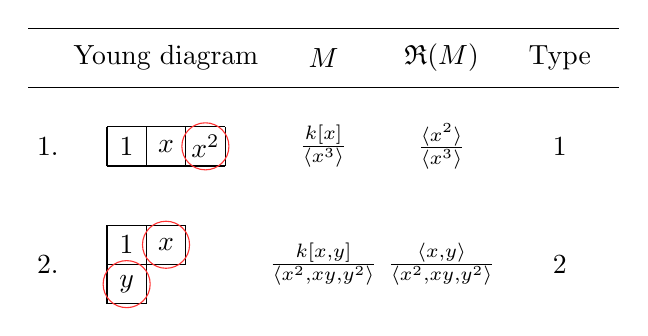
\begin{tikzpicture} [scale=0.5]
				\draw[-](0,6) -- (15,6);
				\draw[-](0,7.5) -- (15,7.5);	 		
				\node (P) at (3.5, 6.75) {Young diagram};
				\node (P) at (7.5, 6.75) {\textbf{$M$}};
				\node (P) at (10.5, 6.75) {$\mathfrak{R}(M)$};
				\node (P) at (13.5, 6.75) {Type};
				
				\node (P) at (0.5, 4.5) {1.};
				
				\draw[-](2, 4) -- (5, 4);
				\draw[-](2, 5) -- (5, 5);
				\draw[-] (2, 4) -- (2, 5);
				\draw[-] (5, 4) -- (5, 5);
				\draw[-] (3, 4) -- (3, 5);
				\draw[-] (4, 4) -- (4, 5);
				
				\node (P) at (2.5, 4.5) {1 };
				\node (P) at (3.5, 4.5) {$x$ };
				\node[circle, draw=red!80, inner sep=0pt, minimum size=17pt ] (c) at (4.5,4.5) {$x^2$};
				
				\node (P) at (7.5, 4.5) { $\frac{k[x]} {\langle x^3 \rangle}$};
				
				\node (P) at (10.5, 4.5) { $\frac{\langle x^2 \rangle} {\langle x^3 \rangle}$};
				\node (P) at (13.5, 4.5) {1};
				
				\node (P) at (0.5, 1.5) {2.};
				
				\draw[-](2, 0.5) -- (3, 0.5);
				\draw[-](2, 1.5) -- (4, 1.5);
				\draw[-] (2, 2.5) -- (4, 2.5);
				\draw[-] (3, 0.5) -- (3, 2.5);
				\draw[-] (4, 1.5) -- (4, 2.5);
				\draw[-] (2, 0.5) -- (2, 2.5);
				
				\node (P) at (2.5, 2) {1 };
				\node [circle, draw=red!80, inner sep=0pt, minimum size=17pt] (c) at (3.5, 2)  {$x$};
				\node [circle, draw=red!80, inner sep=0pt, minimum size=17pt] (c) at (2.5, 1)  {$y$};
				
				\node (P) at (7.5, 1.5) { $  \frac{k[x,y]}{\langle x^2, xy, y^2\rangle}$};	
				\node (P) at (10.5, 1.5) { $\frac{\langle  x,y \rangle} {\langle x^2, xy, y^2\rangle}$};
				
				\node (P) at (13.5, 1.5) {2};
				
%				\node (P) at (0.5, -2) {3.};
%				
%				\draw[-](2, -3.5) -- (3, -3.5);
%				\draw[-](2, -2.5) -- (3, -2.5);
%				\draw[-] (2, -1.5) -- (3, -1.5);
%				\draw[-] (2, -0.5) -- (3, -0.5);
%				\draw[-] (2, -3.5) -- (2, -0.5);
%				\draw[-] (3, -3.5) -- (3, -0.5);
%				
%				\node (P) at (2.5, -1) {1 };
%				\node (P) at (2.5, -2) {$y$ };
%				\node [circle, draw=red!80, inner sep=0pt, minimum size=17pt] (c) at (2.5, -3)  {$y^2$};
%				
%				\node (P) at (7.5, -2) { $ \frac{k[y]}{\langle  y^3\rangle} $};
%				
%				\node (P) at (10.5, -2) { $\frac{\langle y^2 \rangle }{\langle y^3 \rangle}$};
%				\node (P) at (13.5, -2) {1};
			\end{tikzpicture}$$
			\caption{ $\mathfrak{R}(M)$ and its types for a $3$-dimensional $k$-module $M\in \mathfrak{C}$.}
			
			$$	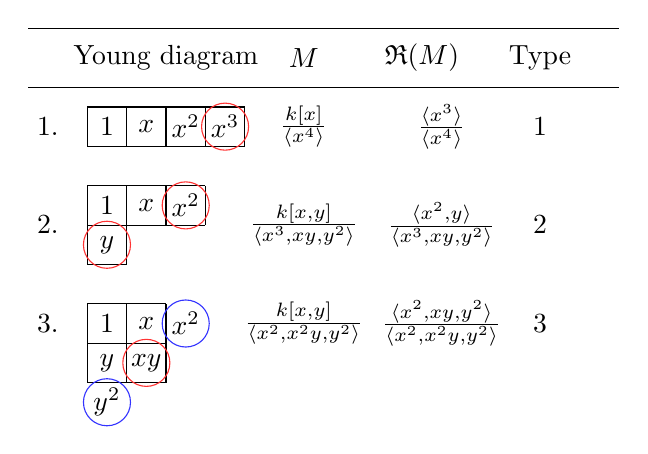
\begin{tikzpicture}[scale=0.5]
				
				\draw[-](0,8) -- (15, 8);
				\draw[-](0,9.5) -- (15,9.5);				
				\node (P) at (3.5, 8.75) {Young diagram};
				\node (P) at (7, 8.75) {$M$};
				\node (P) at (10, 8.75) {$\mathfrak{R}(M)$};
				\node (P) at (13, 8.75) {Type};
				
				\node (P) at (0.5, 7) {1.};
				\draw[-](1.5, 6.5) -- (5.5, 6.5);
				\draw[-](1.5, 7.5) -- (5.5, 7.5);
				\draw[-] (1.5, 6.5) -- (1.5, 7.5);
				\draw[-] (2.5, 6.5) -- (2.5, 7.5);
				\draw[-] (3.5, 6.5) -- (3.5, 7.5);
				\draw[-] (4.5, 6.5) -- (4.5, 7.5);
				\draw[-] (5.5, 6.5) -- (5.5, 7.5);
				
				\node (P) at (2, 7) {1 };
				\node (P) at (3, 7) {$x$ };
				\node (P) at (4, 7) {$x^2$};
				\node [circle, draw=red!80, inner sep=0pt, minimum size=17pt] (c) at (5, 7)  {$x^3$};
				
				\node (P) at (7, 7) { $\frac{k[x]} {\langle x^4 \rangle}$};
				\node (P) at (10.5, 7) { $\frac{\langle x^3 \rangle} {\langle x^4 \rangle}$};
				\node (P) at (13, 7) {1};
				
				\node (P) at (0.5, 4.5) {2.};
				
				\draw[-](1.5, 3.5) -- (1.5, 5.5);
				\draw[-](2.5, 3.5) -- (2.5,5.5);
				\draw[-] (3.5, 4.5) -- (3.5, 5.5);
				\draw[-] (4.5, 4.5) -- (4.5, 5.5);
				\draw[-] (1.5, 5.5) -- (4.5, 5.5);
				\draw[-] (1.5, 4.5) -- (4.5, 4.5);
				\draw[-] (1.5, 3.5) -- (2.5, 3.5);
				
				\node (P) at (2, 5) {1 };
				\node (P) at (3, 5) {$x$ };
				\node [circle, draw=red!80, inner sep=0pt, minimum size=17pt] (c) at (4, 5)  {$x^2$};
				\node [circle, draw=red!80, inner sep=0pt, minimum size=17pt] (c) at (2, 4)  {$y$};
				
				\node (P) at (7, 4.5) { $  \frac{k[x,y]}{\langle x^3, xy, y^2\rangle}$};	
				\node (P) at (10.5, 4.5) { $\frac{\langle  x^2, y \rangle} {\langle x^3, xy, y^2\rangle}$};
				
				\node (P) at (13, 4.5) {2};
				
				\node (P) at (0.5, 2) {3.};
				
				\draw[-](1.5,0.5) -- (3.5, 0.5);
				\draw[-](1.5, 0.5) -- (1.5, 2.5);
				\draw[-] (1.5, 2.5) -- (3.5, 2.5);
				\draw[-] (3.5, 0.5) -- (3.5, 2.5);
				\draw[-] (2.5, 0.5) -- (2.5, 2.5);
				\draw[-] (1.5, 1.5) -- (3.5, 1.5);
				
				\node (P) at (2, 2) {1 };
				\node (P) at (3, 2) {$x$ };
				\node (P) at (2, 1) {$y$};
				%		\node [circle, draw=red] (c) at (2, -0.5) {} ;
				\node [circle, draw=red!80, inner sep=0pt, minimum size=17pt] (c) at (3, 1)  {$xy$};
				\node [circle, draw=blue!80, inner sep=0pt, minimum size=17pt] (c) at (4, 2)  {$x^2$};
				\node [circle, draw=blue!80, inner sep=0pt, minimum size=17pt] (c) at (2, 0)  {$y^2$};
				\node (P) at (7, 2) { $ \frac{k[x, y]}{\langle x^2, x^2y, y^2 \rangle}$};	
				\node (P) at (10.5, 2) { $\frac{\langle x^2, xy, y^2 \rangle}{\langle x^2, x^2y,  y^2 \rangle}$};
				\node (P) at (13, 2) {3};
%				\node (P) at (0.5, -2) {4.};
%				
%				\draw[-](1.5, -4.5) -- (2.5, -4.5);
%				\draw[-](1.5, -4.5) -- (1.5, -1.5);
%				\draw[-] (2.5, -4.5) -- (2.5, -1.5);
%				\draw[-] (3.5, -2.5) -- (3.5, -1.5);
%				\draw[-] (1.5, -1.5) -- (2.5, -1.5);
%				\draw[-] (1.5, -2.5) -- (3.5, -2.5);
%				\draw[-] (1.5, -3.5) -- (2.5, -3.5);
%				\draw[-] (1.5, -1.5) -- (3.5, -1.5);
%				
%				\node (P) at (2, -2.) {1 };
%				\node [circle, draw=red!80, inner sep=0pt, minimum size=17pt] (c) at (3, -2)  {$x$};
%				\node (P) at (2, -3.) {$y$};
%				\node [circle, draw=red!80, inner sep=0pt, minimum size=17pt] (c) at (2, -4)  {$y^2$};
%				
%				\node (P) at (7, -2) { $ \frac{k[x, y]}{\langle x^2, xy, y^3 \rangle}$};	
%				\node (P) at (10.5, -2) { $\frac{\langle x, y^2 \rangle}{\langle x^2, xy, y^3 \rangle}$};
%				\node (P) at (13, -2) {2};
%				
			\end{tikzpicture}$$
		\caption{ $\mathfrak{R}(M)$ and its types for a 4-dimensional $k$-module $M \in \mathfrak{C}$.}
		\end{figure}
		\begin{figure}[H]

			$$	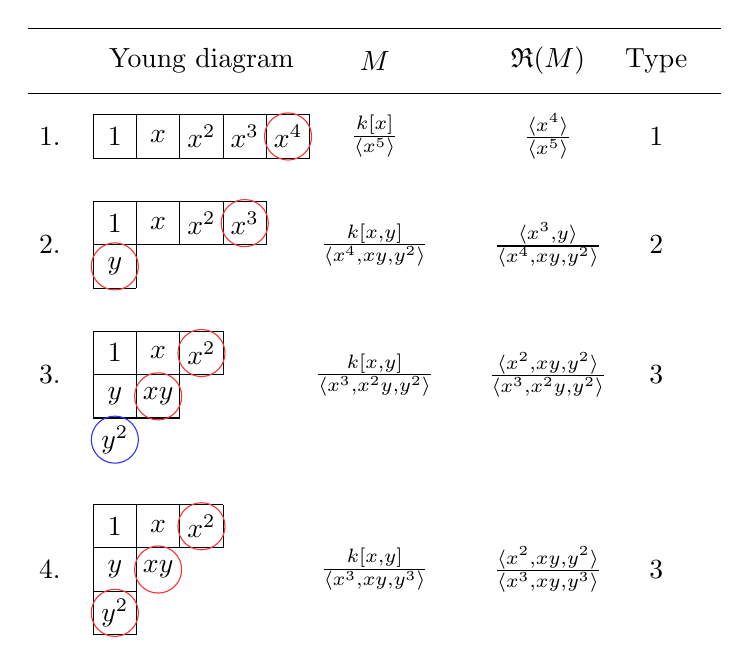
\begin{tikzpicture}[scale=0.55]
				\draw[-](0,13) -- (16,13);
				\draw[-](0,14.5) -- (16,14.5);
				
				\node (P) at (4, 13.75) {Young diagram};
				\node (P) at (8, 13.75) {$M$};
				\node (P) at (12, 13.75) {$\mathfrak{R}(M)$};
				\node (P) at (14.5, 13.75) {Type};
				
				\node (P) at (0.5, 12) {1.};
				
				\draw[-](1.5, 11.5) -- (6.5, 11.5);
				\draw[-](1.5, 11.5) -- (1.5, 12.5);
				\draw[-] (1.5, 12.5) -- (6.5, 12.5);
				\draw[-] (6.5, 11.5) -- (6.5, 12.5);
				\draw[-] (2.5, 11.5) -- (2.5, 12.5);
				\draw[-] (3.5, 11.5) -- (3.5, 12.5);
				\draw[-] (4.5, 11.5) -- (4.5, 12.5);
				\draw[-](5.5,11.5) -- (5.5,12.5);
				
				\node (P) at (2, 12) {1 };
				\node (P) at (3, 12) {$x$ };
				\node (P) at (4, 12) {$x^2$};
				\node (P) at (5, 12) {$x^3$};
				\node [circle, draw=red!80, inner sep=0pt, minimum size=17pt] (c) at (6, 12)  {$x^4$};
				\node (P) at (8, 12) { $\frac{k[x]} {\langle x^5 \rangle}$};
				\node (P) at (12, 12) { $\frac{\langle x^4 \rangle} {\langle x^5 \rangle}$};
				\node (P) at (14.5, 12) {1};
				
				\node (P) at (0.5, 9.5) {2.};
				
				\draw[-](1.5, 8.5) -- (2.5, 8.5);
				\draw[-](1.5, 8.5) -- (1.5,10.5);
				\draw[-] (1.5, 10.5) -- (5.5, 10.5);
				\draw[-] (5.5, 9.5) -- (5.5, 10.5);
				\draw[-] (4.5, 9.5) -- (4.5, 10.5);
				\draw[-] (2.5, 8.5) -- (2.5, 10.5);
				\draw[-] (1.5, 9.5) -- (5.5, 9.5);
				\draw[-] (3.5, 9.5) -- (3.5, 10.5);
				
				\node (P) at (2, 10) {1 };
				\node (P) at (3, 10) {$x$ };
				\node (P) at (4, 10) {$x^2$};
				\node [circle, draw=red!80, inner sep=0pt, minimum size=17pt] (c) at (5, 10)  {$x^3$};
				\node [circle, draw=red!80, inner sep=0pt, minimum size=17pt] (c) at (2, 9)  {$y$};
				\node (P) at (8, 9.5) { $  \frac{k[x,y]}{\langle x^4, xy, y^2\rangle}$};	
				\node (P) at (12, 9.5) { $\frac{\langle  x^3, y \rangle} {\langle x^4, xy, y^2\rangle}$};
				\node (P) at (14.5, 9.5) {2};
				
				\node (P) at (0.5, 6.5) {3.};
				
				\draw[-](1.5,5.5) -- (3.5, 5.5);
				\draw[-](1.5, 5.5) -- (1.5, 7.5);
				\draw[-] (1.5, 7.5) -- (4.5, 7.5);
				\draw[-] (2.5, 7.5) -- (2.5, 5.5);
				\draw[-] (3.5, 7.5) -- (3.5, 5.5);
				\draw[-] (1.5, 6.5) -- (4.5, 6.5);
				\draw[-] (4.5, 6.5) -- (4.5, 7.5);
				
				\node (P) at (2, 7) {1 };
				\node (P) at (3, 7) {$x$ };
				\node [circle, draw=red!80, inner sep=0pt, minimum size=17pt] (c) at (4, 7)  {$x^2$};
				\node (P) at (2, 6.) {$y$};
				\node [circle, draw=red!80, inner sep=0pt, minimum size=17pt] (c) at (3, 6)  {$xy$};
				\node [circle, draw=blue!80, inner sep=0pt, minimum size=17pt] (c) at (2, 5)  {$y^2$};
				\node (P) at (8, 6.5) {  $\frac{k[x, y]}{\langle x^3, x^2y, y^2 \rangle}$};	
				\node (P) at (12, 6.5) { $\frac{\langle x^2, xy, y^2 \rangle}{\langle x^3, x^2y, y^2 \rangle}$};
				\node (P) at (14.5, 6.5) {3};
				
				\node (P) at (0.5, 2) {4.};
				
				
				\draw[-](1.5, 0.5) -- (2.5, 0.5);
				\draw[-](1.5, 1.5) -- (2.5, 1.5);
				\draw[-] (1.5, 2.5) -- (4.5, 2.5);
				\draw[-] (1.5, 3.5) -- (4.5, 3.5);
				\draw[-] (1.5, 0.5) -- (1.5, 3.5);
				\draw[-] (2.5, 0.5) -- (2.5, 3.5);
				\draw[-] (3.5, 2.5) -- (3.5, 3.5);
				\draw[-] (4.5, 2.5) -- (4.5, 3.5);
				
				\node (P) at (2, 3) {1 };
				\node (P) at (3, 3.) {$x$ };
				\node [circle, draw=red!80, inner sep=0pt, minimum size=17pt] (c) at (4, 3)  {$x^2$};
				
				\node (P) at (2, 2) {$y$};
				\node [circle, draw=red!80, inner sep=0pt, minimum size=17pt] (c) at (2, 1)  {$y^2$};
				\node [circle, draw=red!80, inner sep=0pt, minimum size=17pt] (c) at (3, 2)  {$xy$};
				
				\node (P) at (8, 2) { $\frac{k[x, y]}{\langle x^3, xy, y^3 \rangle}$};	
				\node (P) at (12, 2) { $\frac{\langle x^2, xy, y^2 \rangle}{\langle x^3, xy, y^3 \rangle}$};
				\node (P) at (14.5, 2) {3};
				

			\end{tikzpicture}$$
			\caption{$\mathfrak{R}(M)$ and its types for a 5-dimensional $k$-module $M \in \mathfrak{C}$.}
		%\end{figure}
		%\begin{figure}[H]
			
			$$	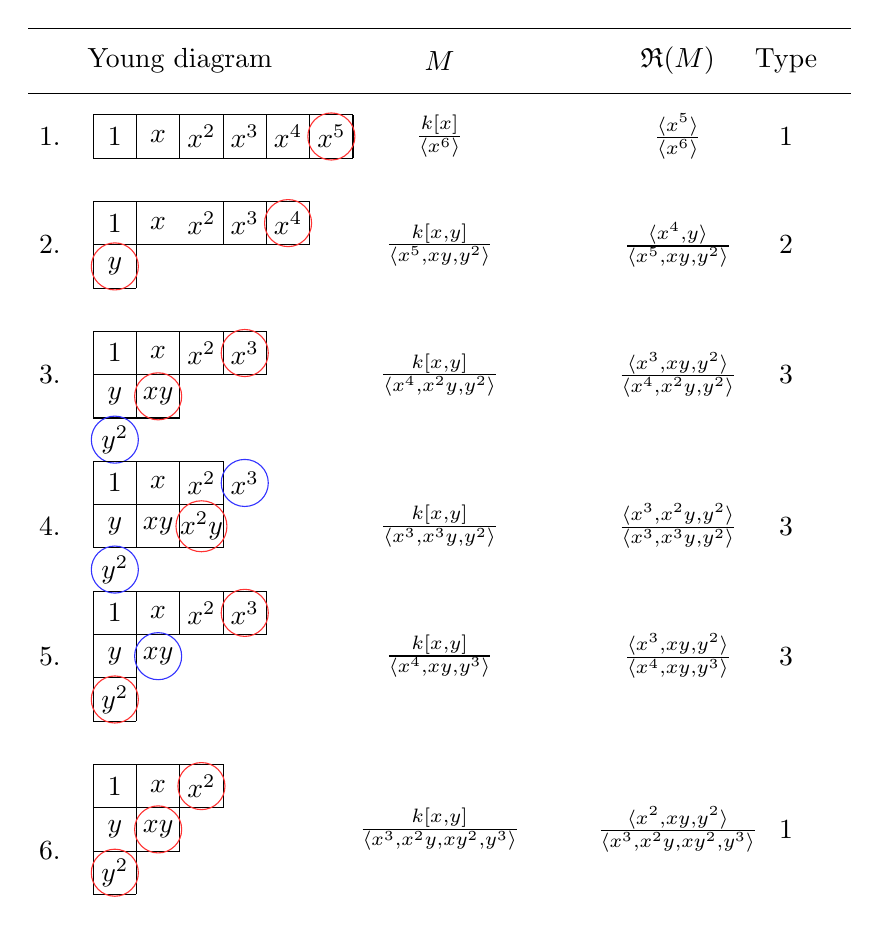
\begin{tikzpicture}[scale=0.55]	
				\draw[-](-3,22.5) -- (16,22.5);		
				\draw[-](-3,21) -- (16,21);
				
				\node (P) at (0.5, 21.75) {Young diagram};
				\node (P) at (6.5, 21.75) {$M$};
				\node (P) at (12, 21.75) {$\mathfrak{R}(M)$};
				\node (P) at (14.5, 21.75) {Type};
				
				\node (P) at (-2.5, 20) {1.};
				
				\draw[-](-1.5, 19.5) -- (-1.5, 20.5);
				\draw[-](-1.5, 19.5) -- (4.5, 19.5);
				\draw[-] (-0.5, 19.5) -- (-0.5, 20.5);
				\draw[-] (0.5, 19.5) -- (0.5, 20.5);
				\draw[-] (1.5, 19.5) -- (1.5, 20.5);
				\draw[-] (2.5, 19.5) -- (2.5, 20.5);
				\draw[-] (3.5, 19.5) -- (3.5, 20.5);
				\draw[-] (4.5, 19.5) -- (4.5, 20.5);
				\draw[-](-1.5,20.5) -- (4.5,20.5);
				
				\node (P) at (-1, 20) {1 };
				\node (P) at (0, 20) {$x$ };
				\node (P) at (1, 20) {$x^2$};
				\node (P) at (2, 20) {$x^3$};
				\node (P) at (3, 20) {$x^4$};
				\node [circle, draw=red!80, inner sep=0pt, minimum size=17pt] (c) at (4, 20)  {$x^5$};
				\node (P) at (6.5, 20) { $\frac{k[x]} {\langle x^6 \rangle}$};
				
				\node (P) at (12, 20) { $\frac{\langle x^5 \rangle} {\langle x^6 \rangle}$};
				\node (P) at (14.5, 20) {1};
				
				\node (P) at (-2.5, 17.5) {2.};
				
				\draw[-](-1.5, 16.5) -- (-0.5, 16.5);
				\draw[-](-1.5, 16.5) -- (-1.5,18.5);
				\draw[-] (-1.5, 18.5) -- (3.5, 18.5);
				\draw[-] (0.5, 18.5) -- (0.5, 18.5);
				\draw[-] (-0.5, 16.5) -- (-0.5, 18.5);
				\draw[-] (-1.5, 17.5) -- (3.5, 17.5);
				\draw[-] (1.5, 17.5) -- (1.5, 18.5);
				\draw[-] (2.5, 17.5) -- (2.5, 18.5);
				\draw[-] (3.5, 17.5) -- (3.5, 18.5);
				
				\node (P) at (-1, 18) {1 };
				\node (P) at (0, 18) {$x$ };
				\node (P) at (1, 18) {$x^2$};
				\node (P) at (2, 18) {$x^3$ };
				\node [circle, draw=red!80, inner sep=0pt, minimum size=17pt] (c) at (3, 18)  {$x^4$};
				\node [circle, draw=red!80, inner sep=0pt, minimum size=17pt] (c) at (-1, 17)  {$y$};
				\node (P) at (6.5, 17.5) { $  \frac{k[x,y]}{\langle x^5, xy, y^2 \rangle}$};	
				\node (P) at (12, 17.5) { $\frac{\langle  x^4, y \rangle} {\langle x^5, xy, y^2\rangle}$};
				\node (P) at (14.5, 17.5) {2};
				
				\node (P) at (-2.5, 14.5) {3.};
				
				
				\draw[-](-1.5, 13.5) -- (0.5,13.5);
				\draw[-] (-1.5, 15.5) -- (2.5, 15.5);
				\draw[-] (-1.5, 14.5) -- (2.5, 14.5);
				\draw[-] (2.5, 14.5) -- (2.5, 15.5);
				
				\draw[-] (-0.5, 13.5) -- (-0.5, 15.5);
				\draw[-] (-1.5, 13.5) -- (-1.5, 15.5);
				
				\draw[-] (0.5, 13.5) -- (0.5, 15.5);
				\draw[-] (1.5, 14.5) -- (1.5, 15.5);
				\node (P) at (-1, 15) {1 };
				\node (P) at (0, 15) {$x$ };
				\node (P) at (-1, 14) {$y$ };
				\node (P) at (1, 15) {$x^2$};
				\node [circle, draw=red!80, inner sep=0pt, minimum size=17pt] (c) at (2, 15)  {$x^3$};
				\node [circle, draw=blue!80, inner sep=0pt, minimum size=17pt] (c) at (-1, 13)  {$y^2$};
				\node [circle, draw=red!80, inner sep=0pt, minimum size=17pt] (c) at (0, 14)  {$xy$};
				\node (P) at (6.5, 14.5) {  $\frac{k[x, y]}{\langle x^4, x^2y, y^2 \rangle}$};	
				\node (P) at (12, 14.5) { $\frac{\langle x^3, xy, y^2 \rangle}{\langle x^4, x^2y, y^2 \rangle}$};
				\node (P) at (14.5, 14.5) {3};
				
				\node (P) at (-2.5, 8) {5.};
				
				\draw[-](-1.5, 6.5) -- (-0.5, 6.5);
				\draw[-](-1.5, 7.5) -- (-0.5,7.5);
				\draw[-] (-1.5, 8.5) -- (2.5, 8.5);
				\draw[-] (-1.5, 9.5) -- (2.5, 9.5);
				\draw[-] (-1.5, 6.5) -- (-1.5, 9.5);
				\draw[-] (-0.5, 6.5) -- (-0.5, 9.5);
				\draw[-] (2.5, 8.5) -- (2.5, 9.5);
				\draw[-] (1.5, 8.5) -- (1.5, 9.5);
				\draw[-] (0.5, 8.5) -- (0.5, 9.5);
				
				\node (P) at (-1, 9) {1 };
				\node (P) at (0, 9) {$x$ };
				\node (P) at (1, 9) {$x^2$};
				\node [circle, draw=red!80, inner sep=0pt, minimum size=17pt] (c) at (2, 9)  {$x^3$};
				\node (P) at (-1, 8) {$y$};
				\node [circle, draw=red!80, inner sep=0pt, minimum size=17pt] (c) at (-1, 7)  {$y^2$};
				\node [circle, draw=blue!80, inner sep=0pt, minimum size=17pt] (c) at (0, 8)  {$xy$};
				
				\node (P) at (6.5, 8) {  $\frac{k[x, y]}{\langle x^4, xy, y^3 \rangle}$};	
				\node (P) at (12, 8) { $\frac{\langle x^3, xy, y^2 \rangle}{\langle x^4, xy, y^3\rangle}$};
				\node (P) at (14.5, 8) {3};
				
				\node (P) at (-2.5,11 ) {4.};
				
				\draw[-](-1.5, 10.5) -- (1.5,10.5);
				\draw[-] (-1.5, 11.5) -- (1.5, 11.5);
				\draw[-] (-1.5, 12.5) -- (1.5, 12.5);
				\draw[-] (-1.5, 10.5) -- (-1.5, 12.5);
				\draw[-] (-0.5, 10.5) -- (-0.5, 12.5);
				\draw[-] (0.5, 10.5) -- (0.5, 12.5);
				\draw[-] (1.5, 10.5) -- (1.5, 12.5);
				
				\node (P) at (-1, 12) {1 };
				\node (P) at (0, 12) {$x$ };
				\node (P) at (1, 12) {$x^2$};
				\node [circle, draw=blue!80, inner sep=0pt, minimum size=17pt] (c) at (2, 12)  {$x^3$};
				\node (P) at (-1, 11) {$y$};
				\node [circle, draw=blue!80, inner sep=0pt, minimum size=17pt] (c) at (-1, 10)  {$y^2$};
				\node (P) at (-0, 11) {$xy$};
				\node [circle, draw=red!80, inner sep=0pt, minimum size=17pt] (c) at (1, 11)  {$x^2y$};
				\node (P) at (6.5, 11) {  $\frac{k[x, y]}{\langle x^3, x^3y, y^2 \rangle}$};	
				\node (P) at (12, 11) { $\frac{\langle x^3, x^2y, y^2 \rangle}{\langle x^3, x^3y, y^2 \rangle}$};
				\node (P) at (14.5, 11) {3};
				
				\node (P) at (-2.5, 3.5) {6.};
				
				\draw[-](-1.5, 2.5) -- (-0.5, 2.5);
				\draw[-](-1.5, 3.5) -- (0.5,3.5);
				\draw[-] (-1.5, 4.5) -- (1.5, 4.5);
				\draw[-] (-1.5, 5.5) -- (1.5, 5.5);
				\draw[-] (-1.5, 2.5) -- (-1.5, 5.5);
				\draw[-] (-0.5, 2.5) -- (-0.5, 5.5);
				\draw[-] (1.5, 4.5) -- (1.5, 5.5);
				\draw[-] (0.5, 3.5) -- (0.5, 5.5);
				
				\node (P) at (-1, 5) {1 };
				\node (P) at (0, 5) {$x$ };
				\node [circle, draw=red!80, inner sep=0pt, minimum size=17pt] (c) at (1, 5)  {$x^2$};
				
				\node (P) at (-1, 4) {$y$};
				\node [circle, draw=red!80, inner sep=0pt, minimum size=17pt] (c) at (0, 4)  {$xy$};
				\node [circle, draw=red!80, inner sep=0pt, minimum size=17pt] (c) at (-1, 3)  {$y^2$};
				
				\node (P) at (6.5, 4) {  $\frac{k[x, y]}{\langle x^3, x^2y,xy^2,y^3 \rangle}$};	
				\node (P) at (12, 4) { $\frac{\langle x^2, xy, y^2 \rangle}{\langle x^3, x^2y,xy^2,y^3 \rangle}$};
				\node (P) at (14.5, 4) {1};
			\end{tikzpicture}$$
				\caption{ $\mathfrak{R}(M)$ and its types for a 6-dimensional $k$-module $M \in \mathfrak{C}$.}
		\end{figure}
		\begin{figure}
			$$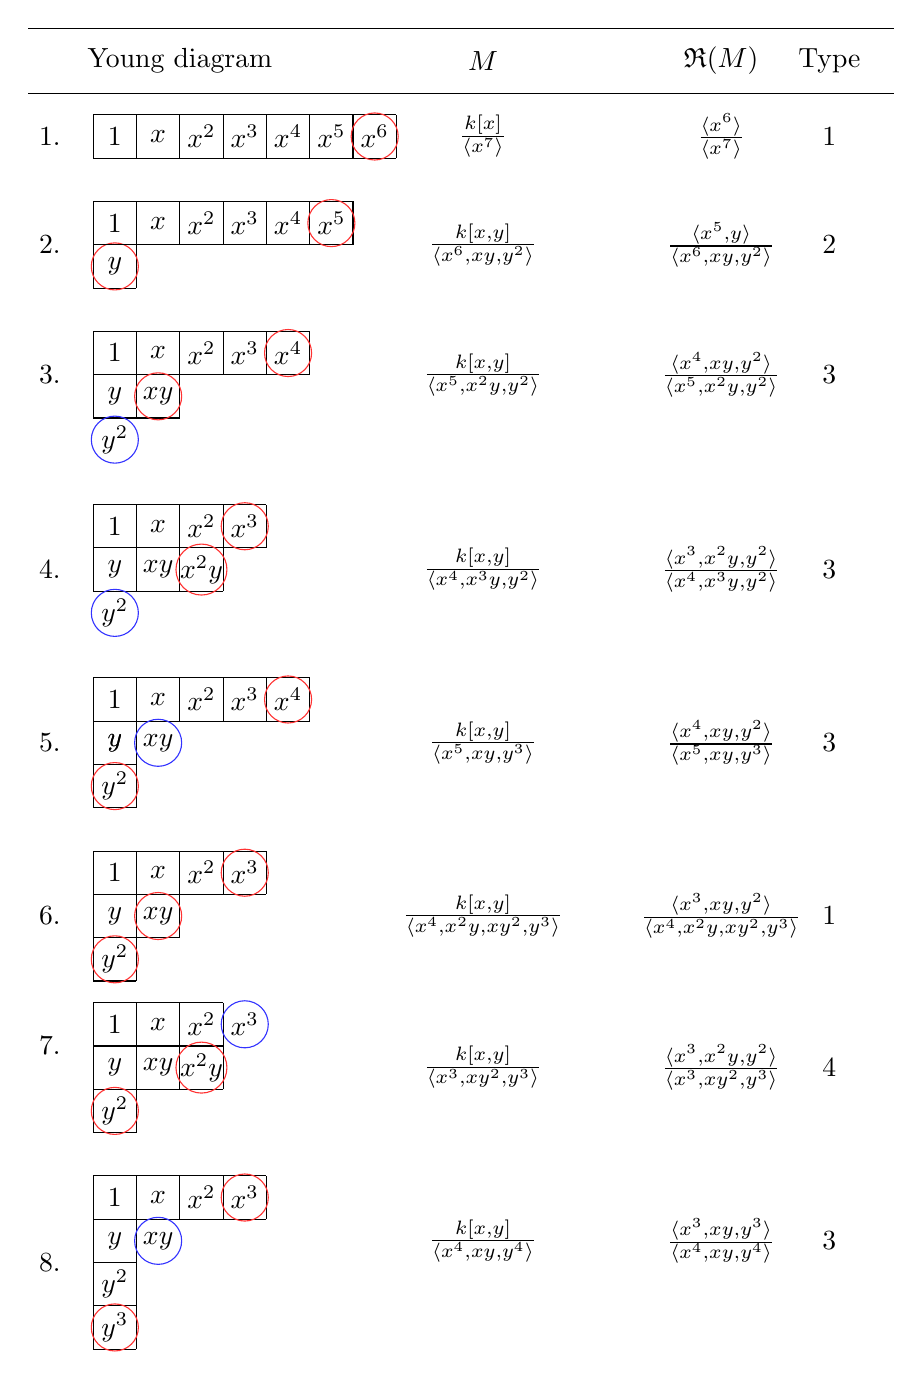
\begin{tikzpicture}[scale=0.55]	
				\draw[-](-3,22.5) -- (17,22.5);		
				\draw[-](-3,21) -- (17,21);
				
				\node (P) at (0.5, 21.75) {Young diagram};
				\node (P) at (7.5, 21.75) {$M$};
				\node (P) at (13, 21.75) {$\mathfrak{R}(M)$};
				\node (P) at (15.5, 21.75) {Type};
				
				\node (P) at (-2.5, 20) {1.};
				
				\draw[-](-1.5, 19.5) -- (-1.5, 20.5);
				\draw[-](-1.5, 19.5) -- (5.5, 19.5);
				\draw[-] (-0.5, 19.5) -- (-0.5, 20.5);
				\draw[-] (0.5, 19.5) -- (0.5, 20.5);
				\draw[-] (1.5, 19.5) -- (1.5, 20.5);
				\draw[-] (2.5, 19.5) -- (2.5, 20.5);
				\draw[-] (3.5, 19.5) -- (3.5, 20.5);
				\draw[-] (4.5, 19.5) -- (4.5, 20.5);
				\draw[-] (5.5, 19.5) -- (5.5, 20.5);
				\draw[-](-1.5,20.5) -- (5.5,20.5);
				
				\node (P) at (-1, 20) {1 };
				\node (P) at (0, 20) {$x$ };
				\node (P) at (1, 20) {$x^2$};
				\node (P) at (2, 20) {$x^3$};
				\node (P) at (3, 20) {$x^4$};
				\node (P) at (4, 20) {$x^5$};
				\node [circle, draw=red!80, inner sep=0pt, minimum size=17pt] (c) at (5, 20)  {$x^6$};
				\node (P) at (7.5, 20) { $\frac{k[x]} {\langle x^7 \rangle}$};
				
				\node (P) at (13, 20) { $\frac{\langle x^6 \rangle} {\langle x^7 \rangle}$};
				\node (P) at (15.5, 20) {1};
				
				\node (P) at (-2.5, 17.5) {2.};
				
				\draw[-](-1.5, 16.5) -- (-0.5, 16.5);
				\draw[-](-1.5, 16.5) -- (-1.5,18.5);
				\draw[-] (-1.5, 18.5) -- (4.5, 18.5);
				\draw[-] (0.5, 18.5) -- (0.5, 18.5);
				\draw[-] (-0.5, 16.5) -- (-0.5, 18.5);
				\draw[-] (-1.5, 17.5) -- (4.5, 17.5);
				\draw[-] (0.5, 17.5) -- (0.5, 18.5);
				\draw[-] (1.5, 17.5) -- (1.5, 18.5);
				\draw[-] (2.5, 17.5) -- (2.5, 18.5);
				\draw[-] (3.5, 17.5) -- (3.5, 18.5);
				\draw[-] (4.5, 17.5) -- (4.5, 18.5);
				\node (P) at (-1, 18) {1 };
				\node (P) at (0, 18) {$x$ };
				\node (P) at (1, 18) {$x^2$};
				\node (P) at (2, 18) {$x^3$ };
				\node (P) at (3, 18) {$x^4$ };
				\node [circle, draw=red!80, inner sep=0pt, minimum size=17pt] (c) at (4, 18)  {$x^5$};
				\node [circle, draw=red!80, inner sep=0pt, minimum size=17pt] (c) at (-1, 17)  {$y$};
				\node (P) at (7.5, 17.5) { $  \frac{k[x,y]}{\langle x^6, xy, y^2 \rangle}$};	
				\node (P) at (13, 17.5) { $\frac{\langle  x^5, y \rangle} {\langle x^6, xy, y^2\rangle}$};
				\node (P) at (15.5, 17.5) {2};
				
				\node (P) at (-2.5, 14.5) {3.};
				
				\draw[-](-1.5, 17.5) -- (-0.5, 17.5);
				\draw[-](-1.5, 13.5) -- (0.5,13.5);
				\draw[-] (-1.5, 15.5) -- (3.5, 15.5);
				\draw[-] (-1.5, 14.5) -- (3.5, 14.5);
				\draw[-] (2.5, 14.5) -- (2.5, 15.5);
				
				\draw[-] (-0.5, 13.5) -- (-0.5, 15.5);
				\draw[-] (-1.5, 13.5) -- (-1.5, 15.5);
				\draw[-] (3.5, 14.5) -- (3.5, 15.5);
				\draw[-] (0.5, 13.5) -- (0.5, 15.5);
				\draw[-] (1.5, 14.5) -- (1.5, 15.5);
				\node (P) at (-1, 15) {1 };
				\node (P) at (0, 15) {$x$ };
				\node (P) at (1, 15) {$x^2$};
				\node (P) at (2, 15) {$x^3$};
				\node [circle, draw=red!80, inner sep=0pt, minimum size=17pt] (c) at (3, 15)  {$x^4$};
				\node (P) at (-1, 14) {$y$};
				\node [circle, draw=blue!80, inner sep=0pt, minimum size=17pt] (c) at (-1, 13)  {$y^2$};
				\node [circle, draw=red!80, inner sep=0pt, minimum size=17pt] (c) at (0, 14)  {$xy$};
				\node (P) at (7.5, 14.5) {  $\frac{k[x, y]}{\langle x^5, x^2y, y^2 \rangle}$};	
				\node (P) at (13, 14.5) { $\frac{\langle x^4, xy, y^2 \rangle}{\langle x^5, x^2y, y^2 \rangle}$};
				\node (P) at (15.5, 14.5) {3};
				
				\node (P) at (-2.5, 6) {5.};
				
				\draw[-](-1.5, 4.5) -- (-0.5,4.5);
				\draw[-] (-1.5, 6.5) -- (3.5,6.5);
				\draw[-] (-1.5, 7.5) -- (3.5, 7.5);
				\draw[-] (-1.5, 4.5) -- (-1.5, 7.5);
				\draw[-] (2.5, 6.5) -- (2.5, 7.5);
				\draw[-] (3.5, 6.5) -- (3.5, 7.5);
				\draw[-] (-0.5, 4.5) -- (-0.5, 7.5);
				\draw[-] (0.5, 6.5) -- (0.5, 7.5);
				%	\draw[-] (1.5, 9.5) -- (1.5, 11.5);
				\draw[-] (-1.5, 5.5) -- (-0.5, 5.5);
				\draw[-] (1.5, 6.5) -- (1.5, 7.5);
				\node (P) at (-1, 7) {1 };
				\node (P) at (0, 7) {$x$ };
				\node (P) at (1, 7) {$x^2$};
				\node (P) at (-1, 6) {$y$};
				\node (P) at (2, 7) {$x^3$};
				\node [circle, draw=red!80, inner sep=0pt, minimum size=17pt] (c) at (3, 7)  {$x^4$};
				\node (P) at (-1, 6) {$y$};
				\node [circle, draw=red!80, inner sep=0pt, minimum size=17pt] (c) at (-1, 5)  {$y^2$};
				\node [circle, draw=blue!80, inner sep=0pt, minimum size=17pt] (c) at (0, 6)  {$xy$};
				\node (P) at (7.5, 6) {  $\frac{k[x, y]}{\langle x^5, xy, y^3 \rangle}$};	
				\node (P) at (13, 6) { $\frac{\langle x^4, xy, y^2 \rangle}{\langle x^5, xy, y^3 \rangle}$};
				\node (P) at (15.5, 6) {3};
				\node (P) at (-2.5, 10) {4.};
				
				\draw[-](-1.5, 9.5) -- (-1.5, 11.5);
				\draw[-](-1.5, 9.5) -- (-0.5,9.5);
				\draw[-] (-1.5, 10.5) -- (2.5, 10.5);
				\draw[-] (-1.5, 9.5) -- (1.5, 9.5);
				\draw[-] (-1.5, 11.5) -- (2.5, 11.5);
				%\draw[-] (-1.5, 4.5) -- (-1.5, 7.5);
				\draw[-] (-0.5, 9.5) -- (-0.5, 11.5);
				\draw[-] (2.5, 10.5) -- (2.5, 11.5);
				\draw[-] (1.5, 9.5) -- (1.5, 11.5);
				\draw[-] (0.5, 10.5) -- (0.5, 11.5);
				\draw[-] (0.5, 9.5) -- (0.5, 11.5);
				
				\node (P) at (-1, 11) {1 };
				\node (P) at (0, 11) {$x$ };
				\node (P) at (1, 11) {$x^2$};
				\node (P) at (0, 10) {$xy$};
				\node [circle, draw=red!80, inner sep=0pt, minimum size=17pt] (c) at (2, 11)  {$x^3$};
				\node (P) at (-1, 10) {$y$};
				\node [circle, draw=blue!80, inner sep=0pt, minimum size=17pt] (c) at (-1, 9)  {$y^2$};
				\node [circle, draw=red!80, inner sep=0pt, minimum size=17pt] (c) at (1, 10)  {$x^2y$};
				
				\node (P) at (7.5, 10) {  $\frac{k[x, y]}{\langle x^4, x^3y, y^2 \rangle}$};	
				\node (P) at (13, 10) { $\frac{\langle x^3, x^2y, y^2 \rangle}{\langle x^4, x^3y, y^2\rangle}$};
				\node (P) at (15.5, 10) {3};
				\node (P) at (-2.5, 2) {6.};
				
				\draw[-](-1.5, 0.5) -- (-0.5, 0.5);
				\draw[-](-1.5, 1.5) -- (0.5,1.5);
				\draw[-] (-1.5, 2.5) -- (2.5, 2.5);
				\draw[-] (-1.5, 3.5) -- (2.5, 3.5);
				\draw[-] (-1.5, 0.5) -- (-1.5, 3.5);
				\draw[-] (-0.5, 0.5) -- (-0.5, 3.5);
				\draw[-] (1.5, 2.5) -- (1.5, 3.5);
				\draw[-] (0.5, 1.5) -- (0.5, 3.5);
				\draw[-] (2.5, 3.5) -- (2.5, 2.5);
				
				\node (P) at (-1, 3) {1 };
				\node (P) at (0, 3) {$x$ };
				\node (P) at (1, 3) {$x^2$ };
				\node [circle, draw=red!80, inner sep=0pt, minimum size=17pt] (c) at (2, 3)  {$x^3$};
				
				\node (P) at (-1, 2) {$y$};
				\node [circle, draw=red!80, inner sep=0pt, minimum size=17pt] (c) at (0, 2)  {$xy$};
				\node [circle, draw=red!80, inner sep=0pt, minimum size=17pt] (c) at (-1, 1)  {$y^2$};
				
				\node (P) at (7.5, 2) {  $\frac{k[x, y]}{\langle x^4, x^2y,xy^2,y^3 \rangle}$};	
				\node (P) at (13, 2) { $\frac{\langle x^3, xy, y^2 \rangle}{\langle x^4, x^2y,xy^2,y^3 \rangle}$};
				\node (P) at (15.5, 2) {1};
				
				\node (P) at (-2.5, -1) {7.};
				
				%\draw[-](-1.5, -10) -- (-0.5, -10);
				\draw[-](-1.5, -3) -- (-0.5,-3);
				\draw[-] (-1.5, -2) -- (1.5, -2);
				\draw[-] (-1.5, -1) -- (1.5, -1);
				\draw[-] (-1.5, 0) -- (1.5, 0);
				\draw[-] (-1.5, -3) -- (-1.5, 0);
				\draw[-] (-0.5, -3) -- (-0.5, 0);
				\draw[-] (-1.5, -1) -- (1.5, -1);
				\draw[-] (1.5, -2) -- (1.5, 0);
				\draw[-] (0.5, -2) -- (0.5, 0);
				
				\node (P) at (-1, -0.5) {1 };
				\node (P) at (0, -0.5) {$x$ };
				\node (P) at (1, -0.5) {$x^2$ };
				\node (P) at (0, -1.5) {$xy$ };
				\node [circle, draw=blue!80, inner sep=0pt, minimum size=17pt] (c) at (2, -0.5)  {$x^3$};
				\node (P) at (-1, -1.5) {$y$};
				\node [circle, draw=red!80, inner sep=0pt, minimum size=17pt] (c) at (1, -1.5)  {$x^2y$};
				\node [circle, draw=red!80, inner sep=0pt, minimum size=17pt] (c) at (-1, -2.5)  {$y^2$};
				
				\node (P) at (7.5, -1.5) {  $\frac{k[x, y]}{\langle x^3, xy^2, y^3 \rangle}$};	
				\node (P) at (13, -1.5) { $\frac{\langle x^3, x^2y, y^2 \rangle}{\langle x^3, xy^2, y^3 \rangle}$};
				\node (P) at (15.5, -1.5) {4};
				
				\node (P) at (-2.5, -6) {8.};
				
				\draw[-](-1.5, -7) -- (-0.5, -7);
				\draw[-](-1.5, -8) -- (-0.5, -8);
				\draw[-](-1.5, -6) -- (-0.5,-6);
				\draw[-] (-1.5, -5) -- (2.5, -5);
				\draw[-] (0.5, -5) -- (0.5, -4);
				\draw[-] (-1.5, -4) -- (2.5, -4);
				\draw[-] (1.5, -5) -- (1.5, -4);
				\draw[-] (2.5, -5) -- (2.5, -4);
				\draw[-] (-1.5, -8) -- (-1.5, -4);
				\draw[-] (-0.5, -8) -- (-0.5, -4);
				\node (P) at (-1, -4.5) {1 };
				\node (P) at (-1, -6.5) {$y^2$};
				\node (P) at (1, -4.5) {$x^2$};
				\node [circle, draw=red!80, inner sep=0pt, minimum size=17pt] (c) at (-1, -7.5)  {$y^3$};
				\node (P) at (0, -4.5) {$x$};
				\node [circle, draw=red!80, inner sep=0pt, minimum size=17pt] (c) at (2, -4.5)  {$x^3$};
				\node [circle, draw=blue!80, inner sep=0pt, minimum size=17pt] (c) at (0, -5.5)  {$xy$};
				\node (P) at (-1, -5.5) {$y$};
				\node (P) at (7.5, -5.5) {  $\frac{k[x, y]}{\langle x^4,xy, y^4 \rangle}$};	
				\node (P) at (13, -5.5) { $\frac{\langle x^3, xy, y^3 \rangle}{\langle x^4, xy, y^4 \rangle}$};
				\node (P) at (15.5, -5.5) {3};
			\end{tikzpicture}$$
		
			\caption{ $\mathfrak{R}(M)$ and its types for a 7-dimensional $k$-module $M \in \mathfrak{C}$.}
		\end{figure}
	\clearpage
		
		Type $4$ modules $M\in \mathfrak{C}$ first show up when $\text{dim}_kM=7$. This is given in Figure $6$. Here, we have a mixture of both, type $2$ as well as type $3$.
		\begin{defn}
			\normalfont
			Let $U$ and $V$ be sets of monomials from the ring $R:=k[x, y]$. We say that elements of $U$ and $V$
			satisfy {\it property $P_V^U$} if for all $a=x^iy^j \in V$, there exists $b=x^py^q \in U$ such that	
			\begin{itemize}
				\item [1.] if $i\leq j$, then $i=p$ and $q=j-1$;
				\item [2.] if $i\geq j$, then $j=q$ and $p=i-1$.
			\end{itemize}
		\end{defn}
		\begin{prop}
			\normalfont
			For any $M\in \mathfrak{C}$, with $\text{dim}_kM\geq 2$ the submodule $\mathfrak{R}(M)$ is non-trivial.
		\end{prop}
		\begin{prf}
			Since for any $M\in \mathfrak{C}$, with $\text{dim}_kM\geq 2$ $\mathfrak{R}(M)=J/I$, where $J$ is a monomial ideal of $R=k[x, y]$, $J\subsetneq k[x, y]$ and therefore $\mathfrak{R}(M)\subsetneq M$.
			By Theorem $2.1$, such $\mathfrak{R}(M)$ is generated by nonconstant terms that appear at the sharp points of the Young diagram corresponding to $M$. Since this set is always non-empty we have $\mathfrak{R}(M) \neq 0$.
		\end{prf}
	\begin{cor}
		\normalfont
		The only reduced $R$-module in $\mathfrak{C}$, is isomorphic to $k$.
	\end{cor}
\begin{prf}
An $R$-module is reduced if and only if $\mathfrak{R}(M)=M$. By Proposition $3.1$, this is possible if $\text{dim}_kM=1$. Since $M\in \mathfrak{C}$, we must have $M=k[x, y]/\langle x, y \rangle \cong k$.
\end{prf}
		
		\begin{thm}
			\normalfont
			For any $M \in \mathfrak{C}$, the submodule $\mathfrak{R}(M)$ takes one of the following forms:
			\begin{itemize}
				\item[] Type $1$: $\mathfrak{R}(M)=A/I$, where generators of $A$ and $I$ satisfy property $P_I^A$.
				
				\item[] Type $2$: $\mathfrak{R}(M)=B/I$, where the generators of $B$ and $I$ except at least one satisfy property $P_I^B$.
				\item[]Type $3$: $\mathfrak{R}(M)=C/I$, where $C$ and $I$ share some generators and the unshared generators satisfy property $P_I^{C^{'}}$, where $C^{'}=C \setminus \{\text{shared generators}\}$.
				\item[]Type $4$: $\mathfrak{R}(M)=D/I$, where $D$ and $I$ share some generators and the unshared generators except at least one satisfy property $P_I^{D^{'}}$, where $D^{'}=D \setminus \{\text{shared generators}\}$.
			\end{itemize}
		\end{thm}
		
		\begin{prf}
			Let $M:=k[x,y]/I\in \mathfrak{R}(M)$. Since by Theorem $2.1$, $\mathfrak{R}(M)$ is a submodule of $M$, it takes the form $J/I$. By Proposition $3.1$, $\mathfrak{R}(M)\neq 0$. Let $S ~(\text{resp}.~G)$ denote the generating set of $J~(\text{resp}.~I)$. If $S\cap G=\emptyset$, then $\mathfrak{R}(M)$ can neither be of type $3$ nor of type $4$. So, if $S\cap G=\emptyset$ and all elements of $S$ and $G$ satisfy property $P_G^S$ then $\mathfrak{R}(M)$ is of type $1$. Otherwise, if $S\cap G=\emptyset$ and some elements of $S$ and $G$ do not satisfy property $P_G^S$, then $\mathfrak{R}(M)$ is of type $2$. Now, suppose that $S\cap G\neq \emptyset$. Then $\mathfrak{R}(M)$ can neither be of type $1$ nor of type $2$. If $S\cap G\neq \emptyset$ and the unshared generators satisfy property $P_G^S$, then $\mathfrak{R}(M)$ is of type $3$. Otherwise, it is of type $4$. These are the only four possibilities.
		\end{prf}
		
		\begin{que}
\normalfont
 Does the type of $\mathfrak{R}(M)$ in general determine the behavior of $M$?
		\end{que}
		\begin{que}
			\normalfont
			Do similar results hold for the ring $R:=k[x, y, z]$, given that three dimensional Young diagrams are well known and relatively easy to manipulate? We hope that even in this case combinatorial methods are handy. For the more general ring $k[x_1, x_2, \cdots,x_n]$ similar combinatorial methods are likely to fail and in this case algebraic techniques may be the appropriate way out.
		\end{que}
		\begin{prop}
			\normalfont
			Let $M:=\frac{k[x,y]}{I}\in\mathfrak{C}$ such that $I:=\langle x^n, x^{n-1}y, \cdots, xy^{n-1}, y^n \rangle$ with $n+1$ distinct generators and $n\geq 3$. Then
			\begin{itemize}
				\item [1.] $\mathfrak{R}(M)$ is of type $1$, and
				\item [2.] $\text{dim}_kM=\frac{n(n+1)}{2}$.
			\end{itemize}
		\end{prop}
		\begin{prf}
			\begin{itemize}
				\item [1.]
				The Young diagram associated to $M$ takes the following shape
				
				$$
				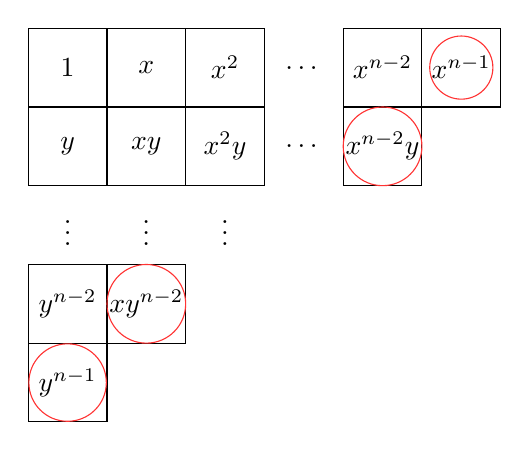
\begin{tikzpicture}
					\draw[-](0, 0) -- (1, 0);
					\draw[-](0, 1) -- (2, 1);
					\draw[-] (0, 2) -- (2, 2);
					\draw[-] (0, 3) -- (3, 3);
					\draw[-] (0, 4) -- (3, 4);
					\draw[-] (0, 5) -- (3, 5);
					\draw[-] (0, 0) -- (0, 2);
					\draw[-] (1, 0) -- (1, 2);
					\draw[-] (2, 1) -- (2, 2);
					\draw[-] (3, 3) -- (3, 5);
					\draw[-] (4, 3) -- (4, 5);
					\draw[-] (5, 3) -- (5, 5);
					\draw[-] (6, 4) -- (6, 5);
					\draw[-] (0, 3) -- (0, 5);
					\draw[-] (1, 3) -- (1, 5);
					\draw[-] (2, 3) -- (2, 5);
					\draw[-] (6, 4) -- (6, 5);
					\draw[-] (4, 5) -- (6, 5);
					\draw[-] (4, 4) -- (6, 4);
					\draw[-] (4, 3) -- (5, 3);
					\node (P) at (0.5, 4.5) {1 };
					\node (P) at (1.5, 4.5) {$x$ };
					\node (P) at (2.5, 4.5) {$x^2$ };
					\node (P) at (3.5, 4.5) {$\dots$} ;
					\node (P) at (4.5, 4.5) {$x^{n-2}$ };
					\node[circle, draw=red!80, inner sep=0pt, minimum size=1pt] ($x^{n-1}$) at (5.5,4.5) {$x^{n-1}$};
					\node (P) at (3.5, 3.5) {$\dots$ };
					\node (P) at (1.5, 3.5) {$xy$ };
					\node (P) at (0.5, 3.5) {$y$ };
					\node (P) at (2.5, 3.5) {$x^2y$ };
					\node[circle, draw=red!80, inner sep=0pt, minimum size=28pt] ($x^{n-2}y$) at (4.5,3.5) {$x^{n-2}y$};
					\node (P) at (0.5, 2.5) {$\vdots$ };
					\node (P) at (1.5, 2.5) {$\vdots$ };
					\node (P) at (2.5, 2.5) {$\vdots$ };
					\node (P) at (0.5, 1.5) {$y^{n-2}$ };
					\node[circle, draw=red!80, inner sep=0pt, minimum size=28pt] ($xy^{n-2}$) at (1.5,1.5) {$xy^{n-2}$};
					\node[circle, draw=red!80, inner sep=0pt, minimum size=28pt] ($y^{n-1}$) at (0.5,0.5) {$y^{n-1}$};
					
				\end{tikzpicture}$$
				The ideal $J$ generated by elements at the sharp points of this Young diagram is $\langle x^{n-1}, x^{n-2}y, \cdots, xy^{n-2}, y^{n-1}\rangle$ which has $n$ distinct generators. Thus, $\mathfrak{R}(M)=\frac{J}{I}$, which is the structure of type $1$ modules.
				\item [2.] Identify each square in the Young diagram with a green dot at the top left corner of the square. We get
				$$
				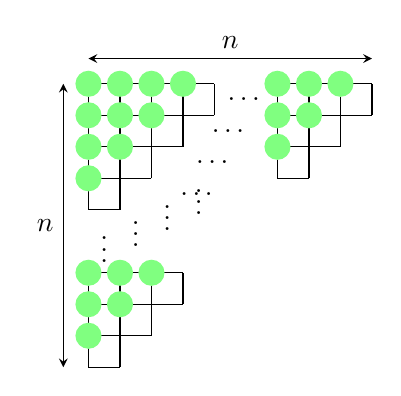
\begin{tikzpicture}[scale=0.4]
					\draw[-](0, -1) -- (1, -1);
					\draw[-](0, 0) -- (2, 0);
					\draw[-](0, 1) -- (3, 1);
					\draw[-] (0, 2) -- (3, 2);
					
					\draw[-] (0, 4) -- (1, 4);
					\draw[-] (0, 5) -- (2, 5);
					\draw[-] (0, 6) -- (3, 6);
					\draw[-] (0, 7) -- (4, 7);
					\draw[-] (0, 8) -- (4, 8);
					
					\draw[-] (6, 8) -- (9, 8);
					\draw[-] (6, 7) -- (9, 7);
					\draw[-] (6, 6) -- (8, 6);
					\draw[-] (6, 5) -- (7, 5);
					
					\draw[-] (0, -1) -- (0, 2);
					\draw[-] (0, 4) -- (0, 8);
					
					\draw[-] (1, -1) -- (1, 2);
					\draw[-] (1, 4) -- (1, 8);
					
					\draw[-] (2, 0) -- (2, 2);
					\draw[-] (2, 5) -- (2, 8);
					
					\draw[-] (3, 1) -- (3, 2);
					\draw[-] (3, 6) -- (3, 8);
					
					\draw[-] (4, 7) -- (4, 8);
					\draw[-] (6, 5) -- (6, 8);
					\draw[-] (7, 5) -- (7, 8);
					\draw[-] (8, 6) -- (8, 8);
					\draw[-] (9, 7) -- (9, 8);
					
					\node (P) at (0.5, 3) {$\vdots$} ;
					\node (P) at (1.5, 3.5) {$\vdots$ };
					\node (P) at (2.5, 4) {$\vdots$ };
					\node (P) at (3.5, 4.5) {$\vdots$ };
					
					\node (P) at (5, 7.5) {$\dots$} ;
					\node (P) at (4.5, 6.5) {$\dots$ };
					\node (P) at (4, 5.5) {$\dots$ };
					\node (P) at (3.5, 4.5) {$\dots$ };
					\draw(0,8) node[fill=green!50, circle]{};
					\draw(1,8) node[fill=green!50, circle]{};
					\draw(2,8) node[fill=green!50, circle]{};
					\draw(3,8) node[fill=green!50, circle]{};
					
					\draw(6,8) node[fill=green!50, circle]{};
					\draw(7,8) node[fill=green!50, circle]{};
					\draw(8,8) node[fill=green!50, circle]{};
					
					\draw(0,7) node[fill=green!50, circle]{};
					\draw(1,7) node[fill=green!50, circle]{};
					\draw(2,7) node[fill=green!50, circle]{};
					\draw(6,7) node[fill=green!50, circle]{};
					\draw(7,7) node[fill=green!50, circle]{};
					
					\draw(0,6) node[fill=green!50, circle]{};
					\draw(1,6) node[fill=green!50, circle]{};
					\draw(6,6) node[fill=green!50, circle]{};
					
					\draw(0,5) node[fill=green!50, circle]{};
					\draw(0,2) node[fill=green!50, circle]{};
					\draw(1,2) node[fill=green!50, circle]{};
					\draw(2,2) node[fill=green!50, circle]{};
					\draw(0,1) node[fill=green!50, circle]{};
					\draw(1,1) node[fill=green!50, circle]{};
					\draw(0,0) node[fill=green!50, circle]{};
					
					\draw[stealth-stealth] (-.8,-1) -- (-.8,8) node[midway,above,left] {$n$};
					\draw[stealth-stealth] (0,8.8) -- (9,8.8) node[midway,above] {$n$};
					
				\end{tikzpicture}$$
				
				
				The dots when combined form shapes of triangles and their numbers form a sequence of triangle numbers, namely; $1, 3, 6, 10, 15, 21,\cdots$ whose sum of first $n$ terms is given by $\frac{n(n+1)}{2}$, see \cite{ross2019dicuil}. Since these dots are in a one-to-one correspondence with the squares of the Young diagram, which are also in a one-to-one correspondence with the generators of $M$, $\text{dim}_kM=\frac{n(n+1)}{2}$.
			\end{itemize}
		\end{prf}
		
		
\begin{center}
\begin{figure}[h]
\pgfplotstableread{type-data.txt}{\table}
 
\begin{tikzpicture}
\begin{axis}[
    xmin = 2, xmax = 69,
    ymin = 0, ymax = 100,
    xtick distance = 10,
    ytick distance = 20,
    grid = both,
    minor tick num = 1,
    major grid style = {lightgray},
    minor grid style = {lightgray!25},
    width = \textwidth,
    height = 0.5\textwidth,
    legend cell align = {left},
    legend pos = north east,
    xlabel={Dimension of module},
    ylabel={Percentage share}
]
 
\addplot[olive, very thick] table [x = {x}, y = {T1}] {\table};
 
\addplot[violet, very thick] table [x ={x}, y = {T2}] {\table};
 
\addplot[teal, very thick] table [x = {x}, y = {T3}] {\table};

\addplot[cyan, very thick] table [x = {x}, y = {T4}] {\table};
 
\legend{
    Type 1, 
    Type 2,
    Type 3,
    Type 4
}
 
\end{axis}
 
\end{tikzpicture}
\label{fig:type-data}
\caption{Distribution of types by dimension}
\end{figure}
\end{center}
 
Given the combinatorial structure of these modules and their reduced submodules, one can implement an algorithm to compute the reduced submodule and its type.
Using a computer we can test effectively many examples of 'monomial modules' and can for each dimension compute all possible modules in the category $C$ and the distribution of the types.
We have implemented in python a tool which, given a module in $C$, computes the reduced module and type.
The tool and a user guide can be found at \cite{bunnett2022github}. 
 
Figure \ref{fig:type-data} displays the distribution of types as the dimension increases, up to a maximum dimension of 70.
Using an average laptop, it takes 1000 seconds to carry out all computations (for every module in $C$ from dimension 2 to 69) and the bottleneck is the computation and storage of all Young diagrams.

One sees a clear picture emerging: While type 3 dominates at first, type 4 increases slowly and all others relatively decrease.
We conjecture:???????????????
		
		\section{Geometric interpretation}
		~~~Given a graded ring $R$ and an integer $d$, the graded ring $\bigoplus_{n\geq d}R_n$ is denoted by $R_{\geq d}$. An element $m$ of a graded $R$-module $M$ is {\it torsion} if $R_{\geq s}m=0$ for some integer $s$. The torsion elements in $M$ form a graded submodule which is denoted by $\tau (M)$ and called the {\it torsion submodule} of $M$.	
		\begin{prop}
			\normalfont
			For any $R$-module $M \in \mathfrak{C}$, 
			$\mathfrak{R}(M) \subseteq \tau(M)$,
		\end{prop}
		\begin{prf}
			Given $R=k[x, y], R=k \bigoplus kx \bigoplus ky \bigoplus kx^2 \bigoplus \cdots, R_0=k~ \text{and} ~R_{\geq 1}=\langle x, y \rangle$. By Corollary $2.1$, $R_{\geq 1}\mathfrak{R}(M)=0$, so $\mathfrak{R}(M) \subseteq \tau(M)$.
		\end{prf}
		\begin{paragraph}\noi
			The inclusion $\mathfrak{R}(M) \subseteq \tau(M)$ is in general strict. Take for instance all elements $m$
			that are generated by elements that appear two cells away (both horizontally and vertically)	from the zero of $M$ in the Young diagram corresponding to $M$. Then $\langle x^2, y^2 \rangle m=0$ and $\langle x, y\rangle m\neq 0$. So, $m\in \tau(M)$ but $m\notin \mathfrak{R}(M)$.
		\end{paragraph}
		\begin{paragraph}\noi	
			The Hilbert scheme, $\text {Hilb} ^n(k^2)$ of $n$ points in the plane consists of those ideals $I \subseteq k[x, y]$ for which the quotient $k[x, y]/I$ has dimension $n$ as a vector space over $k$, \cite{miller2005combinatorial}.
		\end{paragraph}
		\begin{prop}
			\normalfont
			If $I \in \text{Hilb} ^n(k^2)$ is a monomial ideal then there exists an ideal $J$ of $k[x, y]$ such that $J \in \text Hilb ^{n-i}(k^2)$ for some specific positive integer $i$ in the range $1 \leq i <n$ and $\mathfrak{R}(M)=\frac{J}{I}$, where $M:=\frac{k[x, y]}{I}$.
		\end{prop}
		\begin{prf}
			If $I \in \text{Hilb} ^n(k^2)$, then by definition of a Hilbert scheme, $\text{dim}(\frac{k[x, y]}{I})=n < \infty$. Let $M=\frac{k[x, y]}{I
			}$. It follows by Theorem $3.1$ that $\mathfrak{R}(M)=\frac{J}{I}$ for some ideal $J \subseteq k[x, y]$ containing $I$. So, $\frac{k[x, y]}{J}$ is another $k[x, y]$-module such that $\text{dim}_k(\frac{k[x, y]}{J})=t<n= \text{dim}_k(\frac{k[x, y]}{I})$. This shows that $J \in \text{Hilb} ^t(k^2)$ and $t=n-i$ for $1\leq i<n$.	
		\end{prf}
		\begin{cor}
			\normalfont
			For any $M\in\mathfrak{C}$, $\mathfrak{R}(M)=J/I$, where $I\in \text{Hilb} ^n(k^2)$ and $J\in \text{Hilb} ^{n-i}(k^2)$, for some specific positive integer $i$ in the range $1 \leq i <n$.
		\end{cor}
		\begin{prf}
			If $M\in \mathfrak{C}$, then $M=k[x,y]/I$ with $I$ a monomial ideal and $\text{dim}_kM=n<\infty$. It follows from the definition of a Hilbert scheme that $I\in \text{Hilb} ^n(k^2)$. The rest follows from Proposition $4.2$.
		\end{prf}
		%\begin{cor}
		%	Let ${\bf x}=x, y$, be elements of $R$ and $M \in \mathfrak{C}$. Then for each $j$, $$H^j(x, y, M) \in \mathfrak{C}_\text{red}$$
		%	
		%\end{cor}
		%\begin{prf}
		%	By \cite[Proposition $6.20$]{iyengar2007twenty}, $\langle x, y \rangle$ annihilates $H^j(x, y, M)$ then, by Corollary $2.3$ $$H^j(x, y, M) \in \mathfrak{C}_\text{red}$$.
		%\end{prf}
		\subsection*{Acknowledgment}
		\begin{paragraph}\noi
			The authors acknowledge support from the International Science Program (ISP), EMS-Simons for Africa and the Eastern Africa Algebra Research Group (EAALG). The authors are grateful to Rikard Bøgvad for pointing out Example $2.1$ to them and to Balazs Szendroi for comments. 
		\end{paragraph}
		
		\addcontentsline{toc}{chapter}{Bibliography}
		\begin{thebibliography}{99}
			\bibitem{agayev2009reduced}Agayev, N., Halicio{\u{g}}lu, S. and Harmanci, A. (2009). On reduced modules, {\it Commun. Fac. Sci. Univ. Ank. Ser. A1 Math. Stat.}, {\bf 58}(1), 9--16.
			%\bibitem{artin1994noncommutative} Artin, M. and Zhang, J. (1994). Noncommutative projective schemes, {\it Adv. Math.}, {\bf 109}(2), 228--287.
			
			\bibitem{bhatt2019prisms} Bhatt, 
			B. and Scholze, P. (2022). Prisms and prismatic cohomology, {\it Ann. of Math}, accepted.
			
			\bibitem{fulton1997young}  Fulton, W. (1997). Young tableaux: with applications to representation theory and geometry, Mathematical Society Student Texts, {\it Cambridge University Press}, Cambridge, {\bf 35}.
			
			\bibitem{fulton1991} Fulton, W. and Harris, J. (1991). Representation theory. A first course. Graduate Texts in Mathematics, {\it Readings in Mathematics}, Springer-verlag, New York, {\bf 129}.
			
			\bibitem{iyengar2007twenty} Iyengar, S. B., Leuschke, G. J., Leykin, A., Miller, C., Miller, E., Singh, A.K. and Walther, U. (2007). Twenty-four hours of local cohomology, {\it Amer. Math. Soc.}, {\bf 87}.
			\bibitem{kimuli2022weakly} Kimuli, P. I. and Ssevviiri, D. (2022).
			Weakly-morphic modules, {\it Rend. Circ. Math. Palermo(2)}, Springer, 1--16.
			\bibitem{kyomuhangi2021generalised}Kyomuhangi, A. and Ssevviiri, D. (2021). Generalized reduced modules, {\it Rend. Circ. Math. Palermo(2)}, Springer, 1-11.		
			\bibitem{kyomuhangi2020locally}Kyomuhangi, A. and Ssevviiri, D. (2020). The locally nilradical for modules over commutative rings, {\it Beitr.  Algebra Geom.}, {\bf 61}(4), 759--769.
			
			\bibitem{lee2004reduced}Lee, T. K. and Zhou, Y. (2004). Reduced modules, 
			rings, modules, algebras and abelian groups, {\it Lecture Notes in Pure and Appl. Math.}, Dekker, New York, {\bf 236}, 365--377.
			
			\bibitem{miller2005combinatorial} Miller, E. and Sturmfels, B. (2005). Combinatorial commutative algebra,  {\it Springer-verlag}, New York, {\bf 227}.
			\bibitem{nakajima1999lectures}Nakajima, H. (2016). More lectures on Hilbert schemes of points on surfaces. Development of moduli theory--Kyoto 2013, 173--205, {\it Adv. Stud. Pure Math}, {\bf 69},
			Math. Soc. Japan [Tokyo].
			\bibitem{nicholson2005morphic} Nicholson, W. K. and Campos, E. S. (2005). Morphic modules,
			{\it Comm. Algebra}, {\bf 33}(8), 2629--2647.
			
			\bibitem{rege2008reduced}Rege, M. B. and Buhphang, A. M. (2008). On reduced modules and rings, {\it Int. Electron. J. Algebra}, {\bf 3}, 58--74.
			
			\bibitem{rohrer2019torsion} Rohrer, F. (2019). Torsion functors, small or large,
			{\it Beitr. Algebra Geom.}, {\bf 60}(2), 233--256.
			\bibitem {ross2019dicuil} Ross, H. E. and Knott, B. I. (2019). Dicuil (9th century) on triangular and square numbers,
			{\it Br. J. Hist. Math.}, Taylor \& Francis, {\bf 34}(2), 79--94.
			
			
			
			\bibitem{schenzel2018completion} Schenzel, P. and Simon, A. M. (2018). Completion, {\v{C}}ech and local homology and cohomology, Interactions between them, {\it Springer Monographs in Mathematics}, Springer, Cham.
			
			\bibitem{ssevviiri2022applications} Ssevviiri, D. (2022). Applications of reduced and coreduced modules I, {\it arXiv preprint arXiv:2205.13241}.
			
			\bibitem {ssevviiri2012structure} Ssevviiri, D. (2012).
			Structure of non-nilpotent elements of some $\mathbb{Z}$-modules, {\it   Int. J. Algebra}, {\bf 6} (13-16), 691--695.
			
			%			\bibitem{ssevviiri2018nilpotent}Ssevviiri, D. (2018). Nilpotent elements control the structure of a module. {\it arXiv preprint arXiv:1812.04320}.
			
			
			\bibitem{yekutieli2021weak} Yekutieli, A. (2021). Weak proregularity, derived completion, adic flatness, and prisms, {\it J. Algebra}, {\bf 583}, 126--152.
			
			
			
			
			
			
			
		\end{thebibliography}
		
	\end{document}